\documentclass[twocolumn]{article}
\usepackage{multicol}
\usepackage[affil-it]{authblk}
\usepackage{amsmath}
\usepackage{tcolorbox}
\usepackage{float}
\makeatletter
\newcommand{\vo}{\vec{o}\@ifnextchar{^}{\,}{}}
\makeatother
\usepackage{graphicx}
\setlength{\parindent}{4mm}
\setlength{\parskip}{0mm}
\renewcommand{\baselinestretch}{1.3}
\begin{document}
%##############################################
%TITLE PAGE
\title{An Analysis of the Fermi Pasta Ulam Problem}
\author{Andrew Crossman}
\affil{Department of Physics and Astronomy, University of Delaware}
\date{March, 22nd 2019}
\maketitle
\newpage
\twocolumn[
\begin{@twocolumnfalse}
%###############################################
%ABSTRACT
%###############################################
\begin{abstract}
 The goal of this paper is to recreate and analyze the classic FPU-$\beta$ model in order to verify FPU's conclusions, and to investigate other fundamental phenomena of the system. Specific phenomena that are explored are: the ergodic transitions that occur at specific values of $\beta_{crit}$ and $\epsilon_{crit}$, the identification of initial conditions that produce super-recurrence, and the structure of Poincare sections that are generated as a result of specific triggers. 
\end{abstract}
\vspace{5mm}
\end{@twocolumnfalse}
]
%###############################################
%INTRODUCTION
%###############################################
\section{Introduction} 
\hspace{\parindent}The Fermi Pasta Ulam (FPU) problem originates from FPU's interest in trying to ''rigorously prove the ergodicity hypothesis which lies at the core
of traditional statistical mechanics.''$^{[1]}$ In order to accomplish this, they decided to simulate the energy sharing functions of a one-dimensional lattice with nonlinear coupling among rigid masses, using one of the very first computers - \textit{MANIAC} at Los Alamos. The simulation consisted of a long chain of particles that were linked by springs that obeyed Hooke’s law in conjunction with a weak nonlinear correction (a quadratic correction in the FPU-$\alpha$ model and a cubic correction in the FPU-$\beta$ model). Given the understanding of statistical mechanics at the time, they predicted that the energy introduced into the lowest frequency mode $\ell=1$ would slowly drift to the other modes, until an equipartition of the total energy was reached as a consequence of ergodicity, provided that the nonlinearity was not extremely small. Initially their prediction held true. The energy dissipated from the n=1 mode into the $\ell=2$, $\ell=3$,... modes over time and reached a quasi-equipartition. However, one day by accident the program was allowed to run much longer and when FPU returned, they noticed that after remaining in a near equipartition state for a while, the energy departed from it. In fact, after 157 periods nearly all of the energy had returned to the initial $\ell=1$ mode! Later calculations performed by faster computers showed that this phenomenon actually repeats many times over, and that a super-recurrence exists when the magnitude of the nonlinear term is less than a certain critical value. In the case that the nonlinear term is greater than this critical value; however, the system behaves ergodicly. Thus, the FPU paradox was born: ''nonlinearity is not sufficient to guarantee the equipartition of energy''$^{[2]}$.
%###############################################
%Methodology
%###############################################
\section{Methodology}
\hspace{\parindent}This paper explores and analyzes the classic FPU-$\beta$ model, which contains 32 identical masses of mass $m$ that are linearly attached by identical springs with spring constant $K$ and an additional nonlinear constant $\beta$. The end points of the 'string' of masses are also stationary and do not move. Given these constraints, the dynamical equation for the $j^{th}$ mass of the system is described as:
\begin{equation}
\begin{split}
	m\frac{d^2x_j}{dt^2}&=K(x_{j+1}-x_j)+\beta(x_{j+1}-x_j)^3\\
	&-K(x_j-x_{j-1})-\beta(x_j-x_{j-1})^3
\end{split}
\end{equation}
Normalizing the equation (see section 3) causes $m$ and $K$ to no longer be present and ensures that the computation relies solely on the initial positions of the masses as defined by the starting mode and the nonlinear $\beta$ value. The normal modes that will be used to describe the system in different states are classified as the eigenvectors of the system in the $\beta=0$ case, which are defined as:
\begin{equation}
	\boldsymbol{e}_{\ell}(j)=\sqrt[]{\frac{2}{N+1}}\sin\left(\frac{\pi\ell}{N+1}j\right)
\end{equation}
where $\ell$ is the normal mode number, $N$ is the total number of masses, and $j$ is the mass number. These eigenvectors form a complete orthonormal basis that can be measured at a particular time $t$ by projecting the location of masses $m_j(t)$ onto them. This contribution per mode is calculated by:
\begin{equation}
	A_{\ell}(t)=\sqrt[•]{\frac{2}{N+1}}\sum_{j=1}^{N}x_j(t)\sin\left(\frac{\pi\ell}{N+1}j\right)
\end{equation}
where $A_{\ell}$ is the eigenvector coefficient of mode $\ell$. The energy contained in each mode can likewise be calculated by utilizing the corresponding eigenvector coefficient $A_{\ell}$ and frequency $\omega_{\ell}$ in the form:
\begin{equation}
	\omega_{\ell} = \left| 2\sin\left(\frac{1}{2}\frac{\pi\ell}{N+1}\right) \right|
\end{equation}
\begin{equation}
	E_{\ell}(t)=\frac{1}{2}\left[ \left(\frac{d}{dt}A_{\ell}(t)\right)^2+\left(\omega_{\ell}A_{\ell}(t)\right)^2 \right]
\end{equation}

In regards to how the aforementioned equations - particularly equation $(1)$ - were used to initialize the system, they were firstly implemented in a Euler-Cromer method  to calculate the positions and velocities of the masses for the first time step. Each step thereafter was then calculated by using the Verlet method instead because of higher degree of accuracy. Furthermore, note that the time steps were set to 0.05 seconds, but smaller steps could have produce better results though it would be at the cost of longer computation time. 
\subsection{Experiment One}
The first experiment was implemented simply to ensure that the system was operating properly by comparing it to other well documented cases involving the classic FPU-$\beta$ model. In order to achieve this, the system was run with an initial starting mode $\ell=1$ and nonlinear factor $\beta=0$ to determine whether any of the initial energy propagated into the other modes over time. Since no nonlinear factor was present in this trial, the energy should not dissipate and instead remain in the starting mode. Assuming that this occurs, the eigenvector coefficients can also be calculated to ensure that the $e_\ell=1$ mode oscillates in time whereas the rest are at a constant zero.
\begin{center}
\begin{figure}[ht!]
\centering
\caption{$\ell=1$ $\beta=0$}
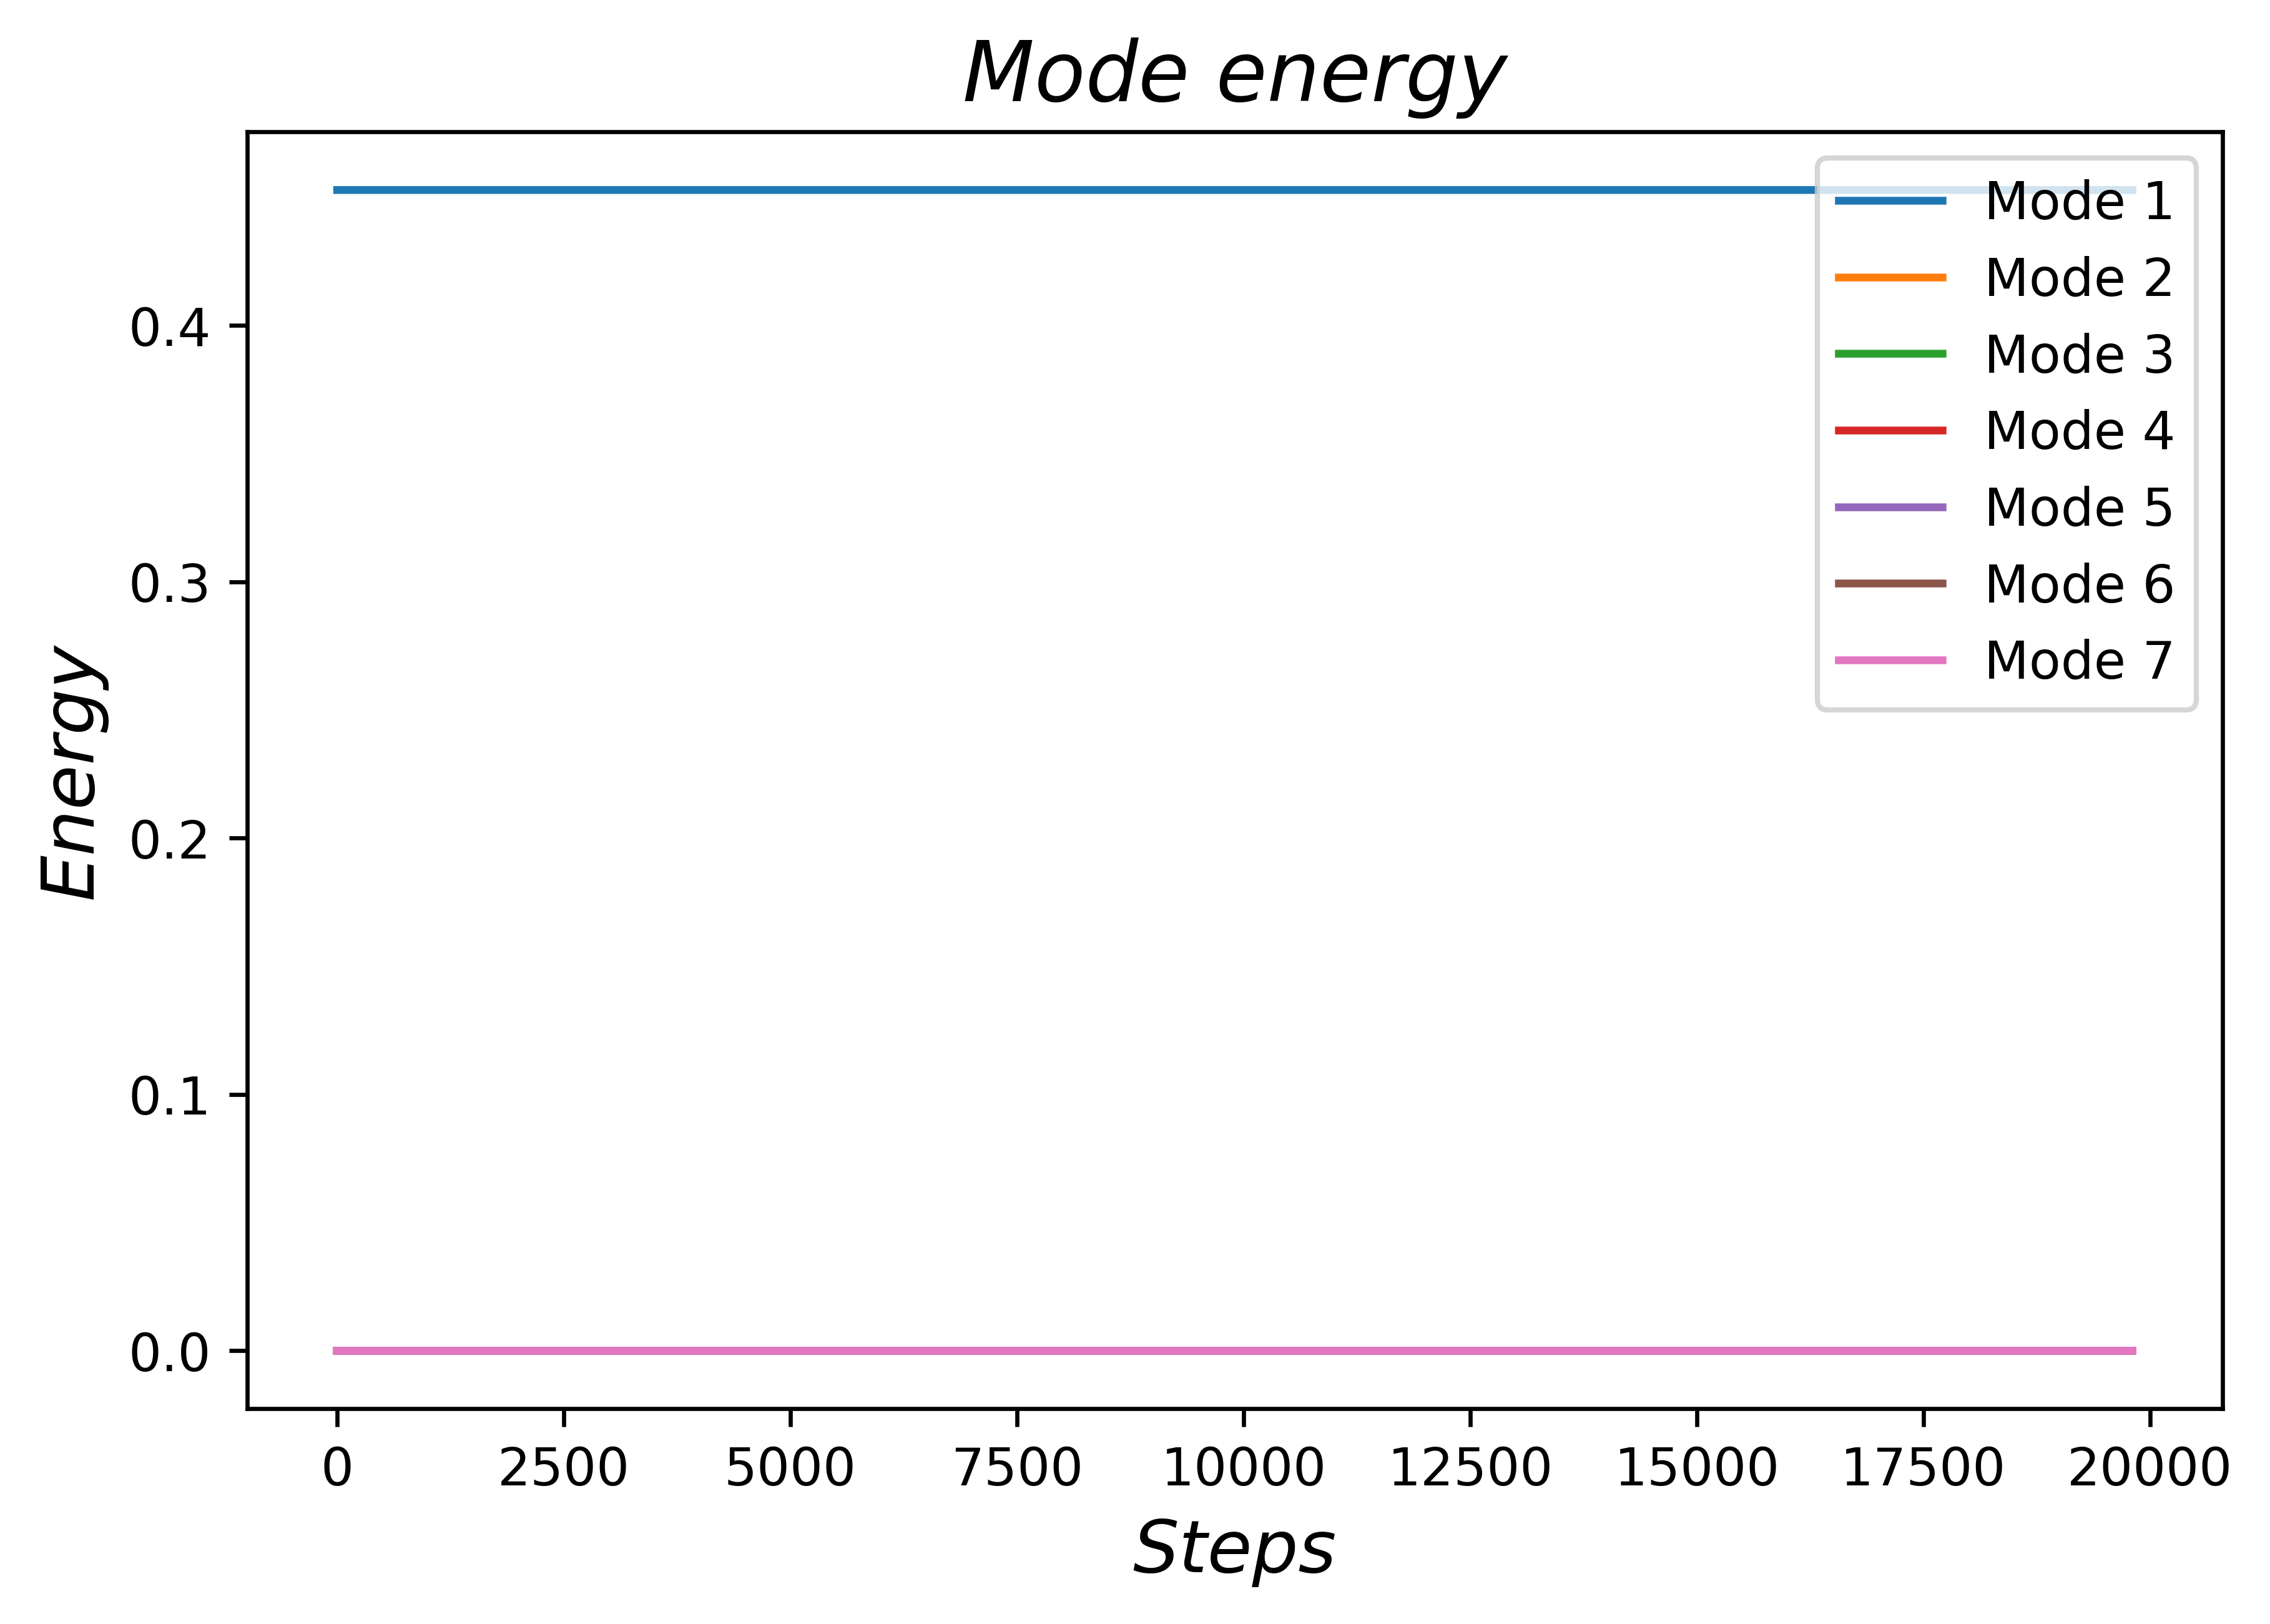
\includegraphics[scale=.55]{EnergiesN=1B=0}
\small{This figure shows that when the system is not exposed to a nonlinear factor that the initial energy is maintained solely in the starting mode and does not dissipate at all into other modes.}
\end{figure}
\end{center}
\subsection{Experiment Two}
The second experiment aimed to demonstrate the FPU paradox once the system was functioning properly in the linear case - confirmed in experiment one. This was performed by initializing the system with the lowest normal mode $\ell=1$ along with a nonlinear factor of $\beta=1$. The energy of the modes were then calculated at each time step and plotted as a function of time to observe whether there was any form of super-recurrence. In the case that there was, the approximate period of this behavior was calculated.
\begin{figure}[ht!]
\centering
\caption{$\ell=1$ $\beta=1$}
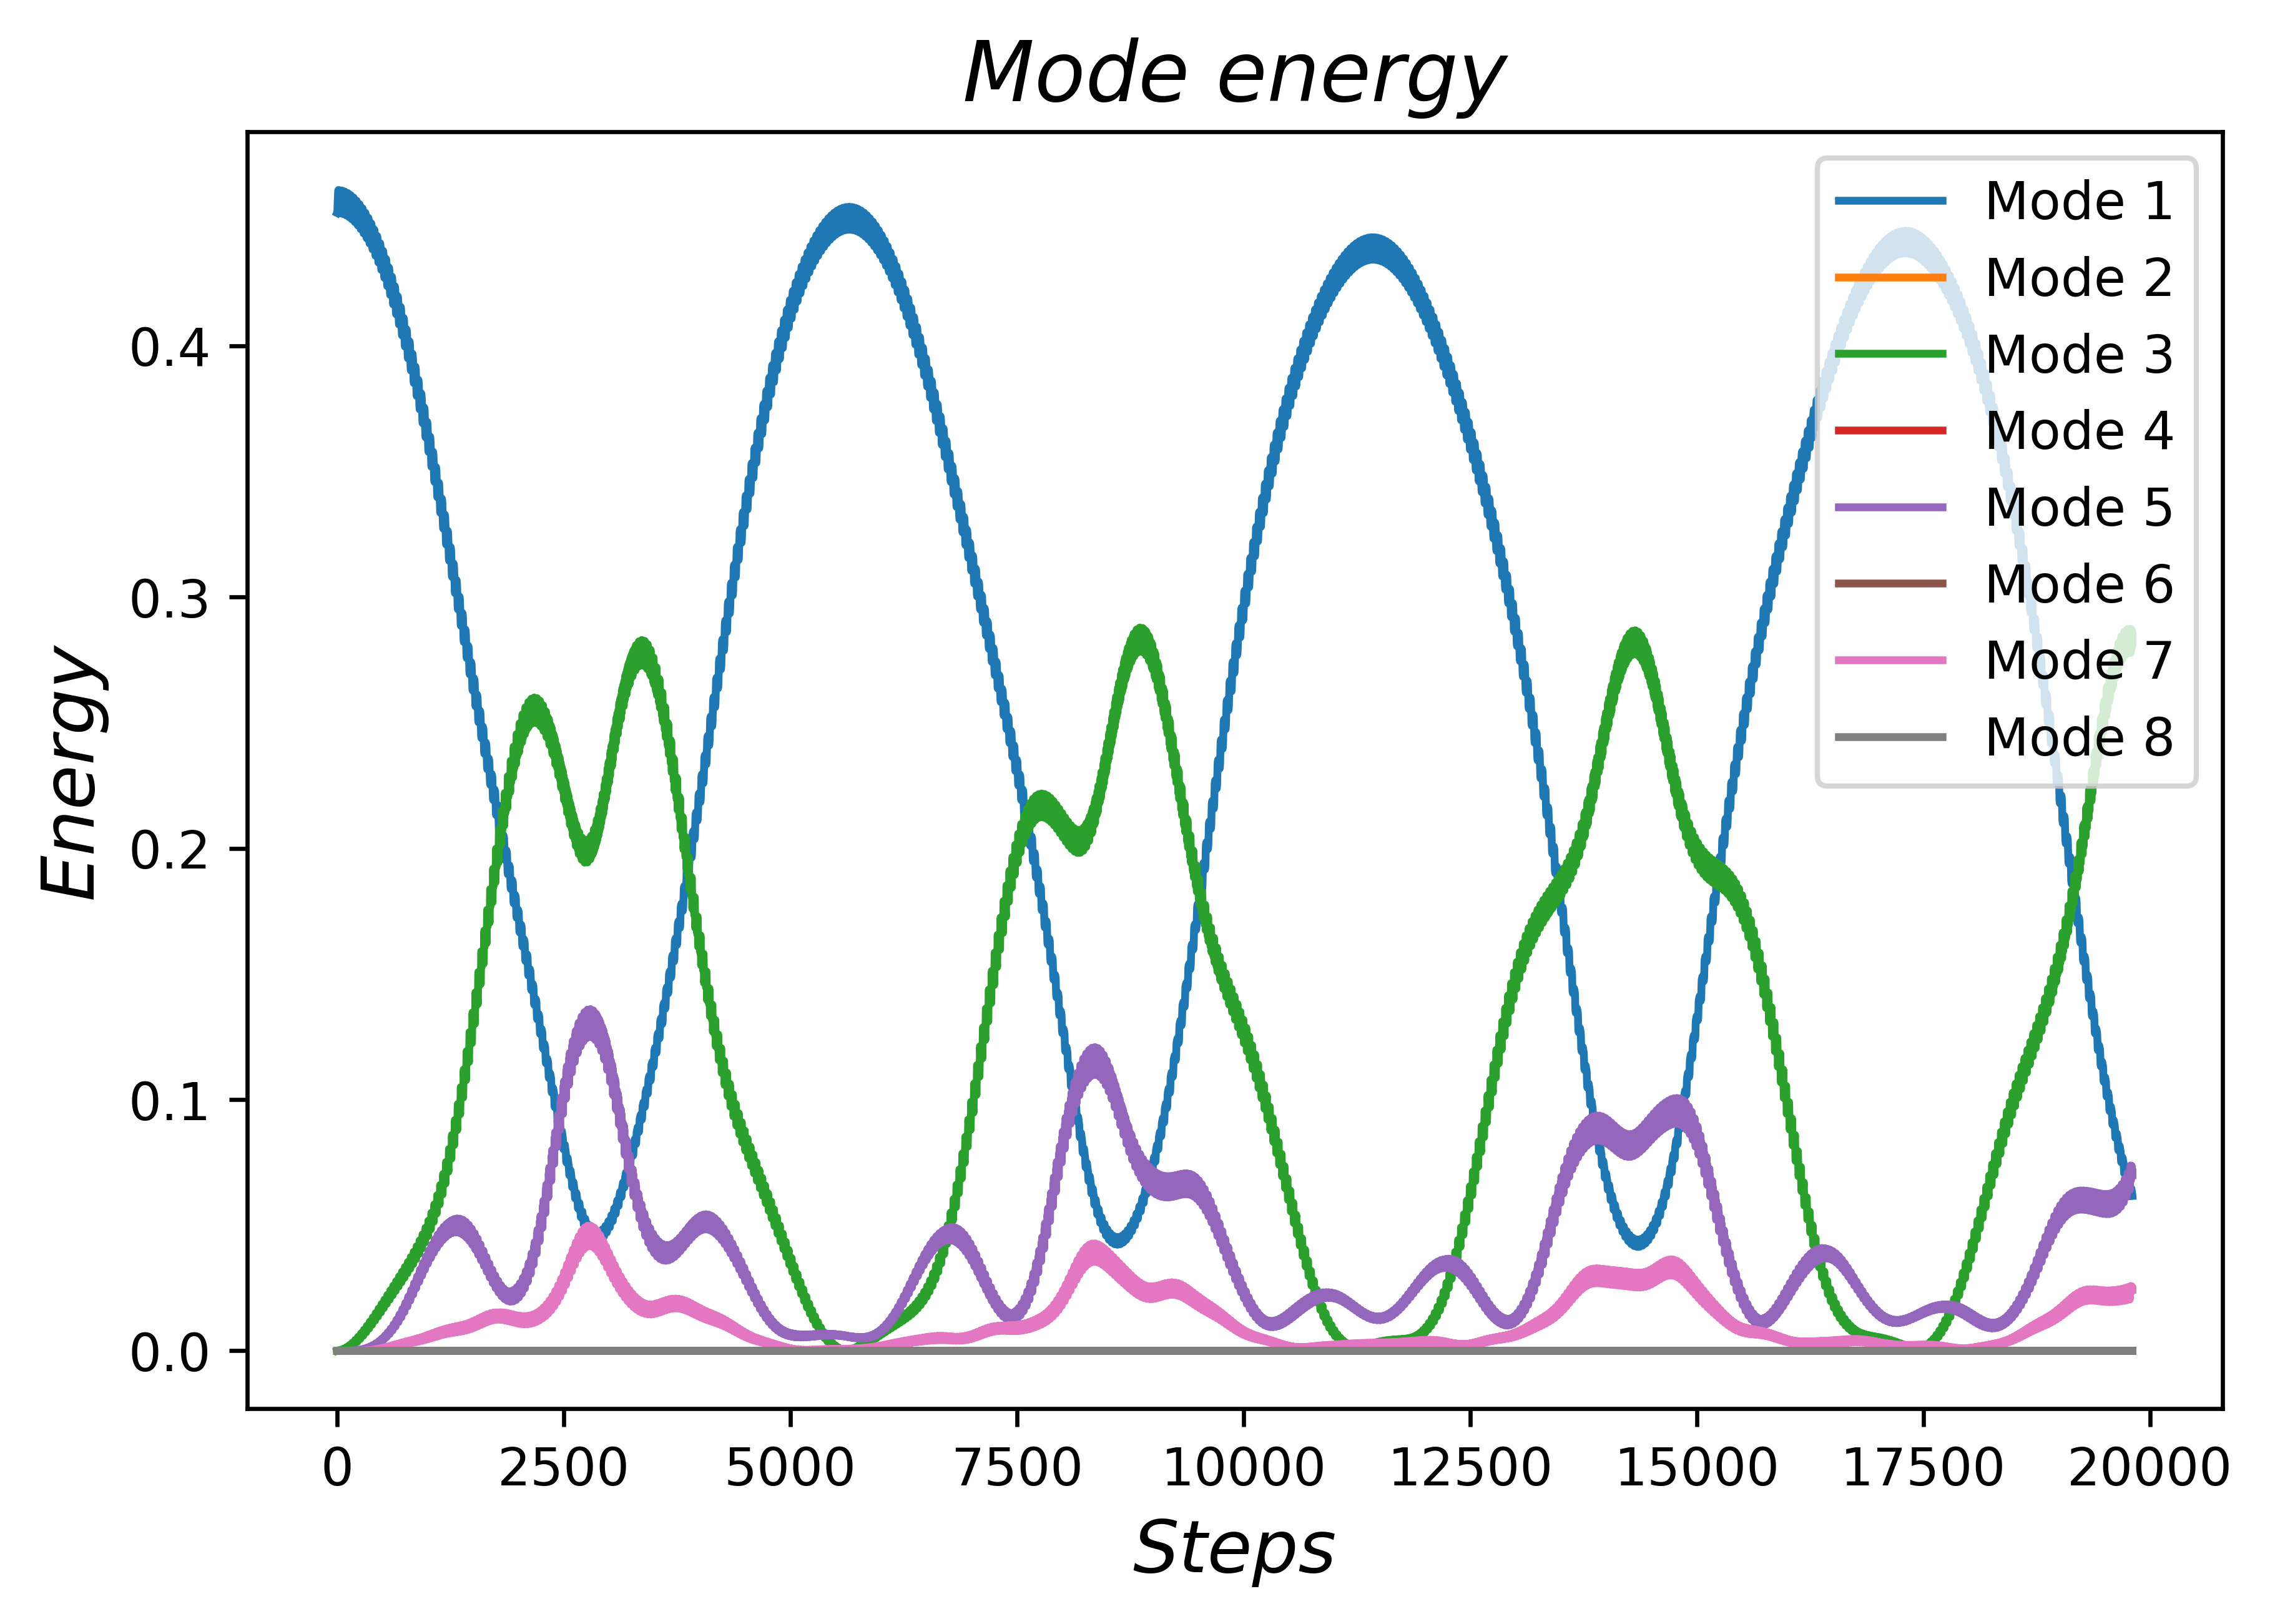
\includegraphics[scale=.55]{EnergiesN=1B=1}
\small{Here the system is introduced to a nonlinearity factor $\beta=1$ which causes the energy to initially dissipate and then return to the $\ell=1$ mode. This phenomena is called super-recurrence.}
\end{figure}
\subsection{Experiment Three}
The third experiment sought to study the transition of the system from a non-ergodic state to an ergodic one. This was achieved in two ways: the first was by examining the standard deviation of the energy across the modes over time ($\sigma_E(t)$) for different $\beta$ values, and the second was by measuring the critical energy per mass ($\epsilon_{crit}$) of the system against its corresponding $\beta$ value. The standard deviation of the energy across the modes over time was calculated using the formula:
\begin{equation}
	\sigma_E(t)=\sqrt{\frac{1}{N-1}\sum_{\ell=1}^{N}\left(E_\ell(t)-\bar{E}_\ell(t)\right)^2}
\end{equation}
In cases where the system is ergodic the plot of $\sigma_E(t)$ vs time depicts an exponential decay and when the system is nonergodic the plot is approximately periodic. The critical energy per mass was calculated by intializing the system at a specific mode and number of particles and determining $\beta_{crit}$ from these quantities; afterwhich, $\beta_{crit}$ was used to find $\epsilon_{crit}$. The critical value of $\beta$ was determined using the formula$^{[1]}$:
\begin{equation}
	3\beta_{crit}\frac{E}{N} \approx 3 \frac{\sqrt{\delta\ell}}{\ell}
\end{equation}
where $E$ is the total energy of the system, $N$ is the number of masses, and $\ell$ is the initializing mode of the system. The critical value of $\epsilon$ was then determined by using the quantities of the system associated with $\beta_{crit}$ in the  form:
\begin{equation}
	\epsilon_{crit}=\frac{E_{\ell0}(t=0)}{N}
\end{equation}
$\epsilon_{crit}$ and its corresponding $\beta_{crit}$ were then plotted agaisnt one another to examine their relationship. Similarly, this experiment was then performed by plotting $\epsilon_{crit}$ against $N$ - where $N$ was used to determine $\beta_{crit}$ - and examining the relationship between these values.
\subsection{Experiment Four}
The fourth experiment aimed to discover other cases of super-recurrence outside of the $\ell=1$ node by applying the critical $\beta$ limit formula used in experiment three to the initializing mode. The system was then run with its new nonlineaity factor and initial mode, and the energies of each mode were plotted over time. When a case was found that displayed some form of super-recurrence, the other modes to which the energy propagated to and the approximate period of the behavior were recorded.
\begin{figure}[ht!]
\centering
\caption{$\ell=1$ $\beta=3$}
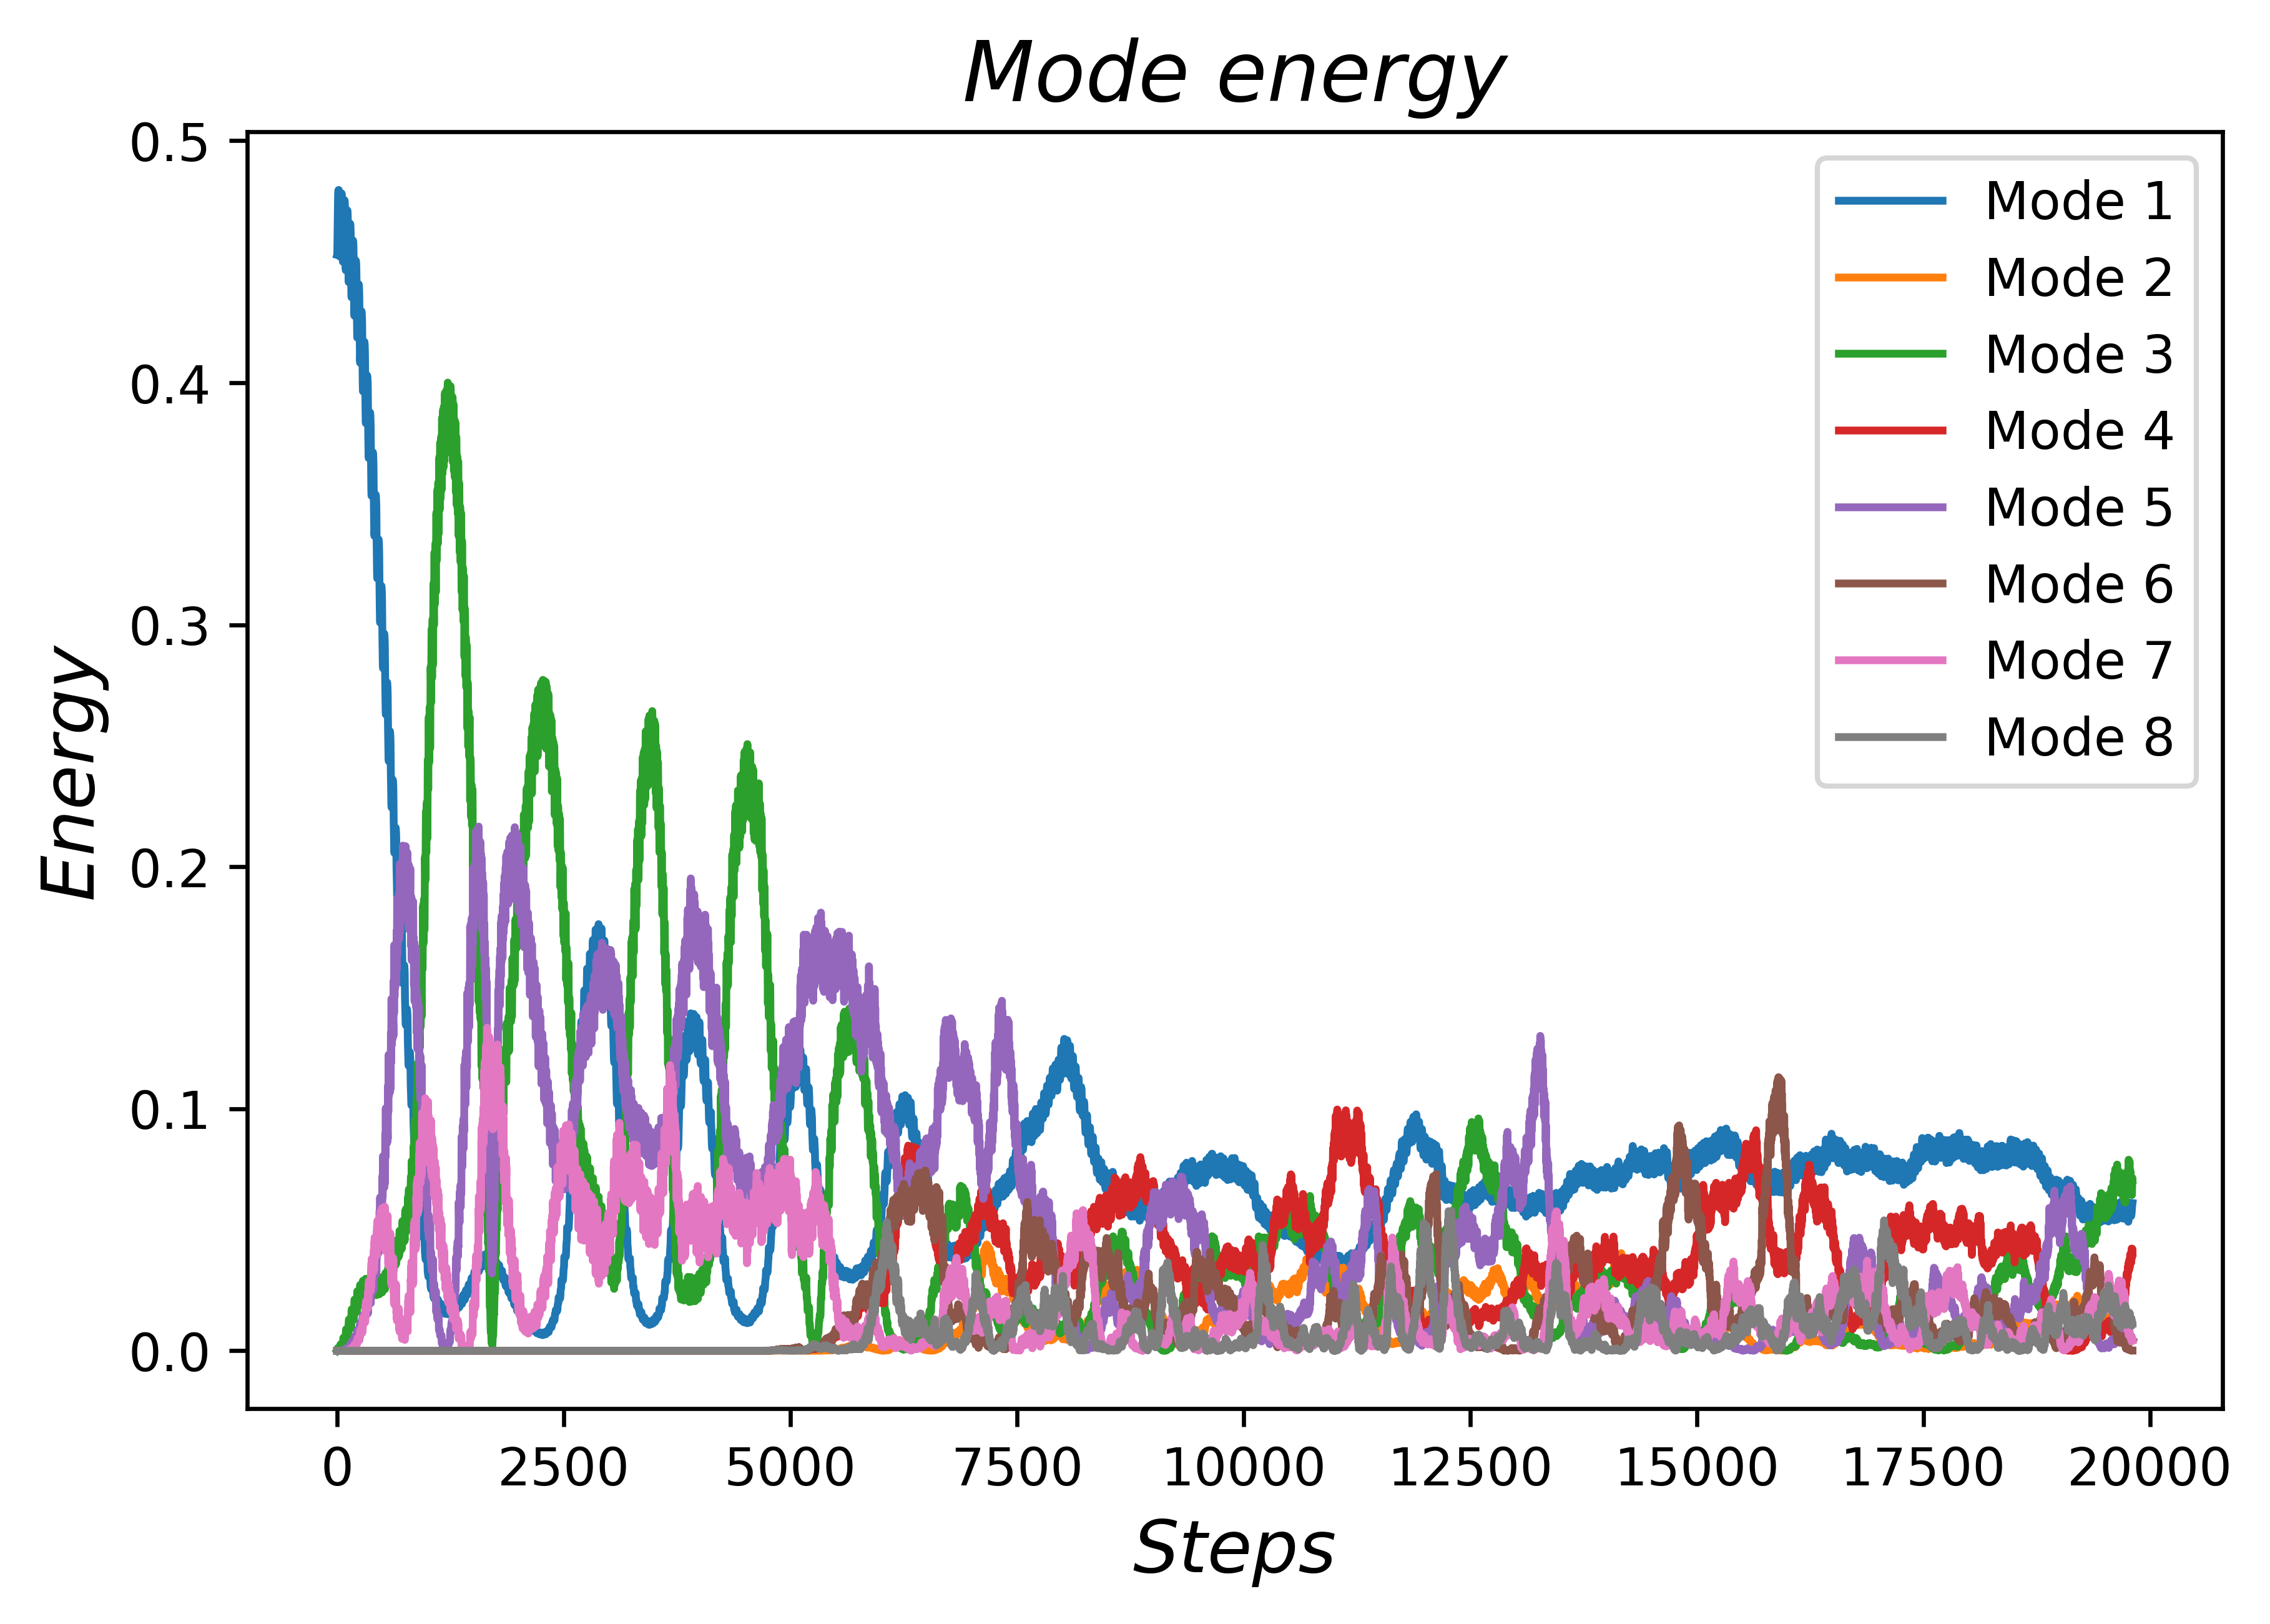
\includegraphics[scale=.53]{EnergiesN=1B=3}
\small{This figure shows the energies for the first 8 normal modes of the system when it is ergodic. Clearly there exists no pattern even after 600 periods of $\omega_{\ell=1}$.}
\end{figure}
\subsection{Experiment Five}
The final experiment aimed at reconstructing the Poincare sections that Giordano produce in \textit{'Computational Physics'} on page 299. These plots were created by plotting $A_{\ell=1}$ against $\frac{d}{dt}A_{\ell=1}$ whenever $A_{\ell=3}=0$ for the cases where the initial mode was $\ell=1$ and the nonlinear factors were $\beta=.3$, $\beta=1$, and $\beta=3$ respectively. Due to the nature of the simulation, however, it should be noted that $A_{\ell=3}$ actually equaling zero at any point of recording data is very unlikely. Hence, the actual data points that were recorded for $A_{\ell=1}$ and $\frac{d}{dt}A_{\ell=1}$ were whenever $-.1<A_{\ell=3}<.1$. Other triggers were also used to compare to the first three Poincare sections.
\begin{figure}[ht!]
\centering
\caption{$\ell=3$ $\beta=0.45$}
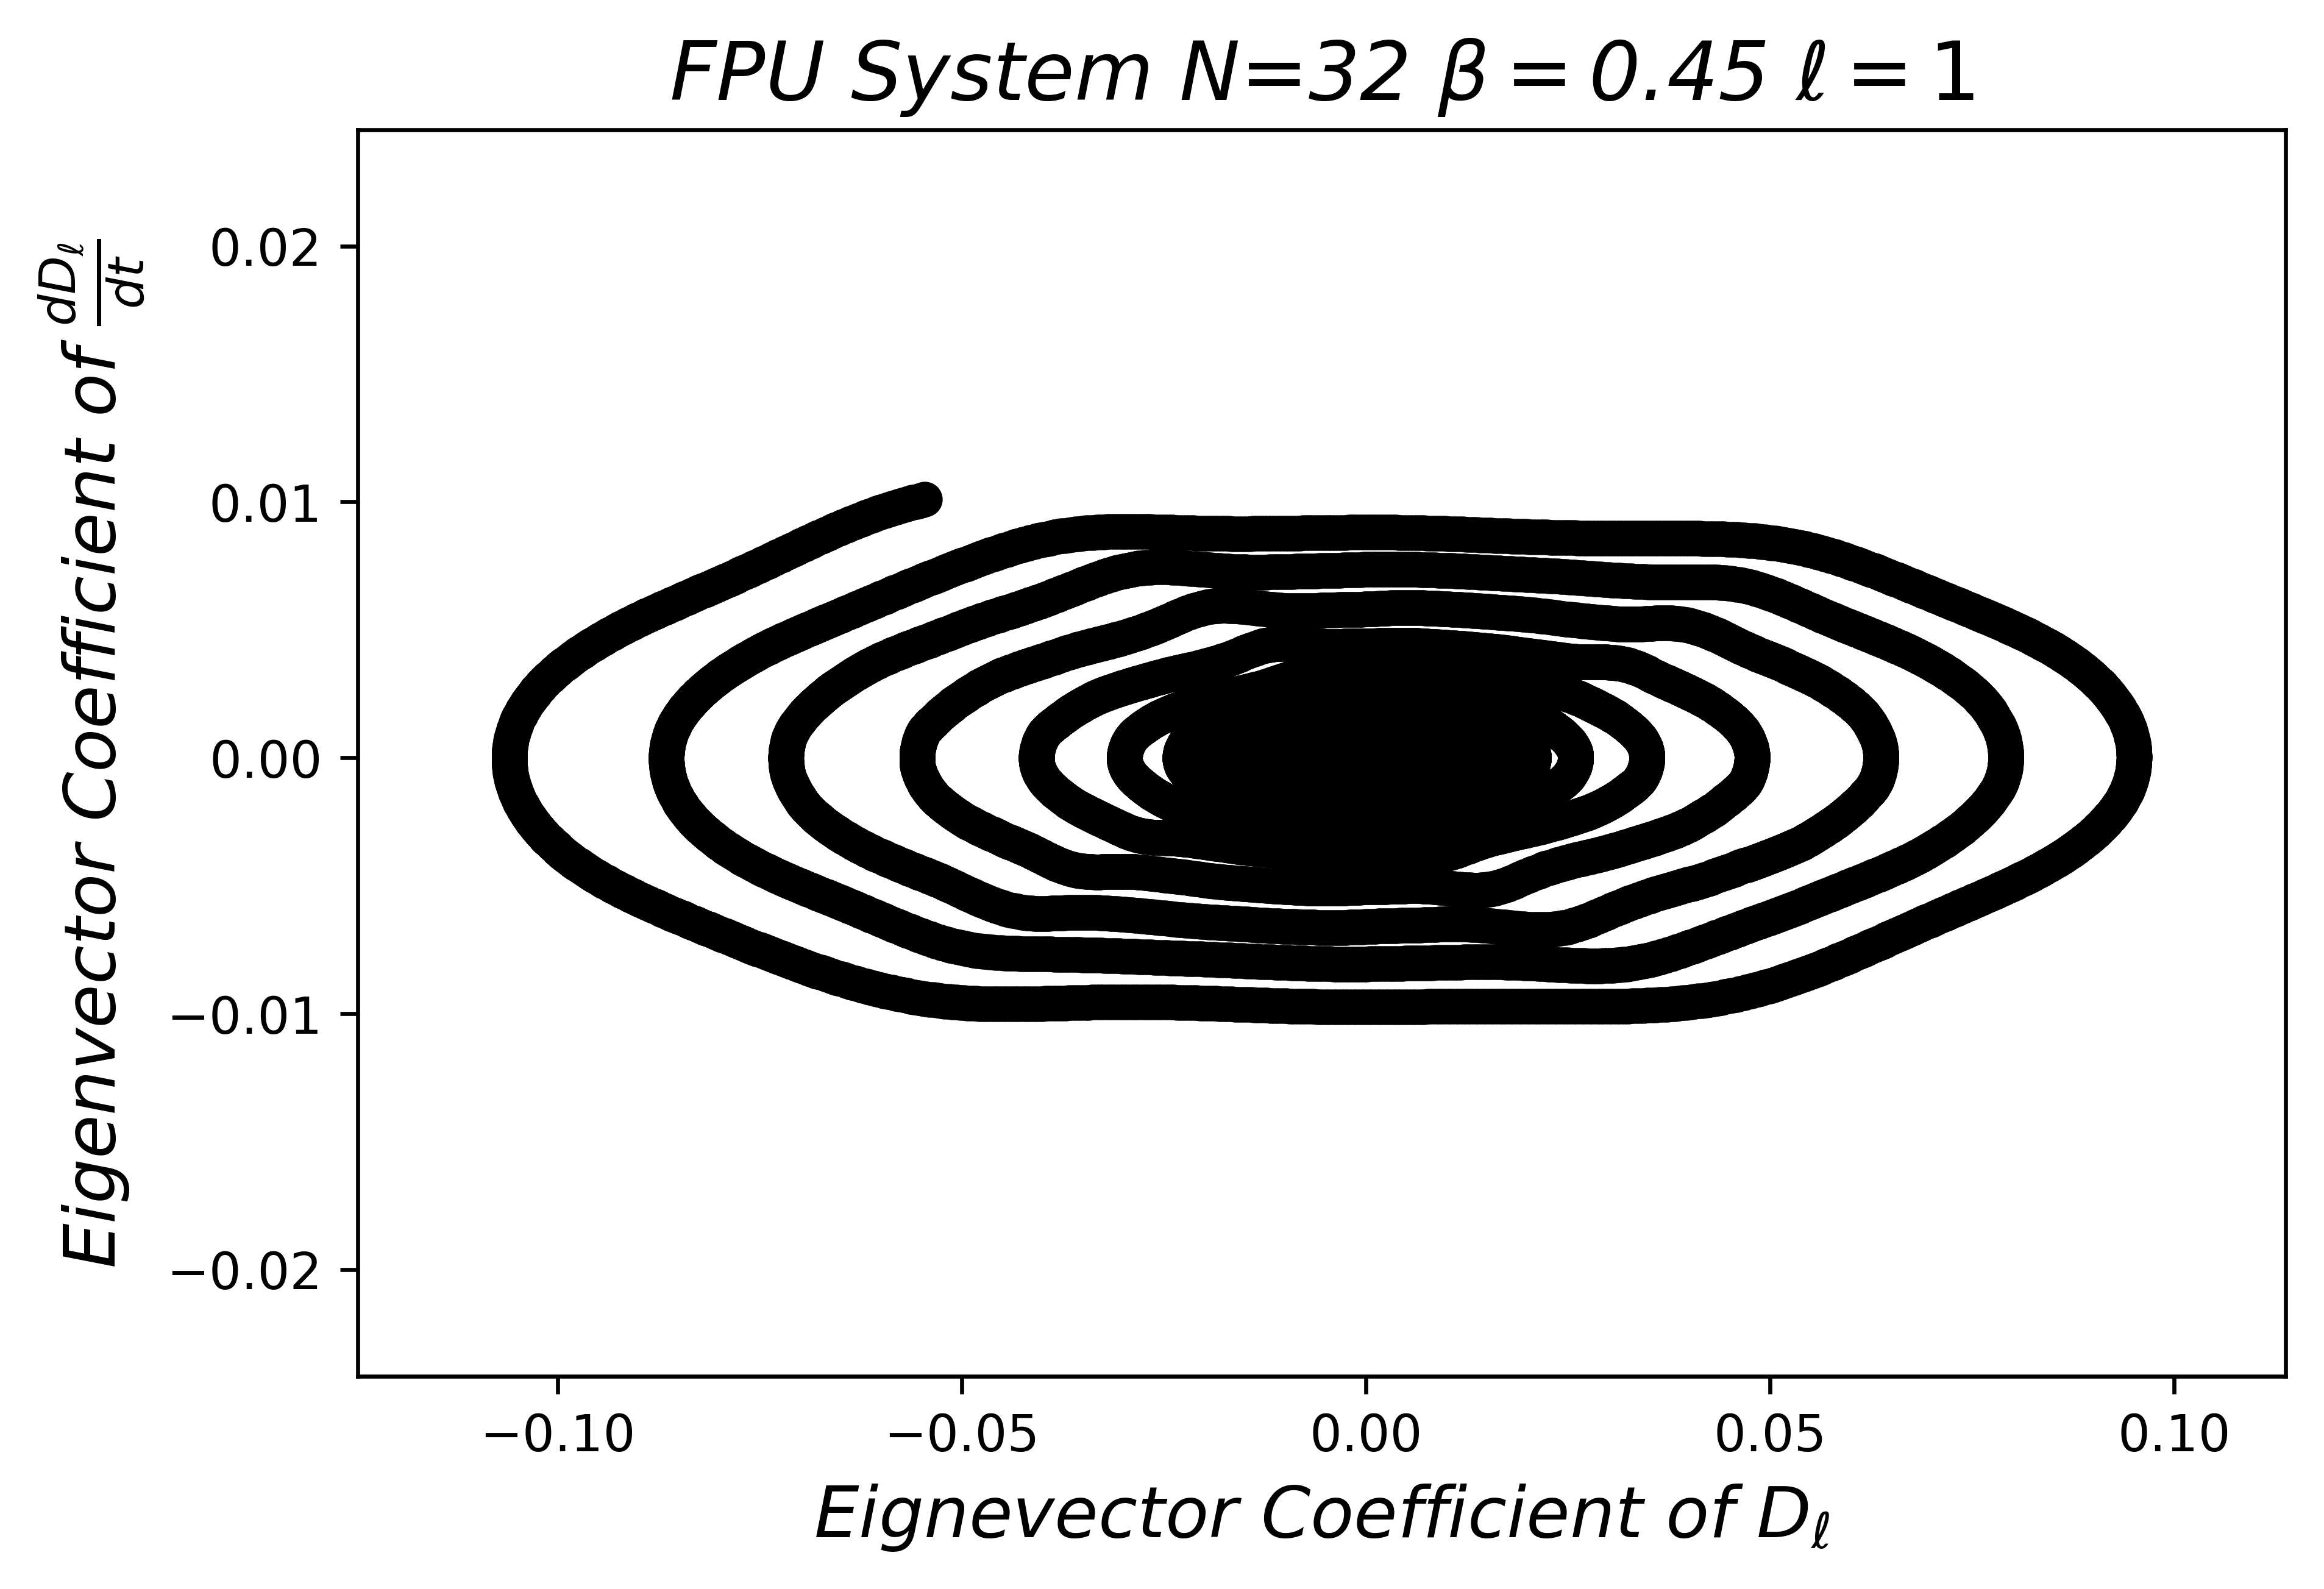
\includegraphics[scale=.55]{Poincare5aN=3B=0}
\small{This figure shows the Poincare section for the system when it is intialized with $\ell=3$ with a nonlinearity factor $\beta=.45$. The data on the plot represents that data points obtained for the trigger $A_{\ell=5}=0$.}
\end{figure}
\section{Normalization}
\hspace{\parindent} Normalizing equation $(1)$ is a key component to producing accurate simulation results in the FPU-$\beta$ model because of both the high frequency of its use (32 times per time-step), and the role it plays in calculating the eigenvectors coefficients and energy in each mode. The normalization is performed as follows:
\begin{equation}
\begin{split}
	m\frac{d^2x_j}{dt^2}&=K(x_{j+1}-x_j)+\beta(x_{j+1}-x_j)^3\\
	&-K(x_j-x_{j-1})-\beta(x_j-x_{j-1})^3
\end{split}
\end{equation}
\begin{equation}
\begin{split}
	\frac{x_0}{t_0^{2}}m\frac{d^2\bar{x}_j}{d\bar{t}^2}=Kx_0(\bar{x}_{j+1}-\bar{x}_j)+\beta x_0^3(\bar{x}_{j+1}-\bar{x}_j)^3\\
	-Kx_0(\bar{x}_j-\bar{x}_{j-1})-\beta x_0^3(\bar{x}_j-\bar{x}_{j-1})^3
\end{split}
\end{equation}
\begin{equation}
\begin{split}
	\frac{d^2\bar{x}_j}{d\bar{t}^2}&=\frac{Kt_0^2}{m}(\bar{x}_{j+1}-\bar{x}_j)+\frac{\beta x_0^2 t_0^2}{m}(\bar{x}_{j+1}-\bar{x}_j)^3\\
	&-\frac{Kt_0^2}{m}(\bar{x}_j-\bar{x}_{j-1})-\frac{\beta x_0^2 t_0^2}{m}(\bar{x}_j-\bar{x}_{j-1})^3
\end{split}
\end{equation}
Now allow...
\begin{equation}
	\frac{Kt_0^2}{m}=1 \implies t_0=\sqrt{\frac{m}{K}}
\end{equation}
\begin{equation}
	\frac{x_0^2t_0^2}{m}=1 \implies x_0=\sqrt{\frac{m}{t_0^2}}=\sqrt{K}
\end{equation}
Hence, normalizing equation $(1)$ yields...
\begin{equation}
\begin{split}
	\frac{d^2\bar{x}_j}{d\bar{t}^2}&=(\bar{x}_{j+1}+\bar{x}_{j-1}-2\bar{x}_j)+\beta(\bar{x}_{j+1}-\bar{x}_j)^3\\
	&-\beta(\bar{x}_j-\bar{x}_{j-1})^3
\end{split}
\end{equation}
where $x_0\bar{x}=x$ and $t_0\bar{t}=t$. It is worth noting that the other equations do not need to be normalized either because they rely on equation $(1)$ which is already normalized or they do not require normalization.
%%%%%%%%%%%%%%%%%%%%%%%%%%%%%%%%%%%
% New Section
%%%%%%%%%%%%%%%%%%%%%%%%%%%%%%%%%%%
\section{Analysis}
\hspace{\parindent}Experiment one successfully confirmed that the system operated exactly as it should when no nonlinear factor was present in the springs. The energy of the system remained in the initialized mode $\ell=1$ throughout all time $t$ - where $t_{max}=\frac{600\pi}{\omega_\ell}$ (see Figure (1)) - and similarly, the eigenvector coefficient for the $\ell=1$ mode oscillated between 10 and -10 at a set period, whereas the other coefficients remained constant at zero. Hence, the system functioned according to the conclusions recorded by FPU and other scientists.
\begin{figure}[ht!]
\centering
\caption{$\ell=2$ $\beta=1$}
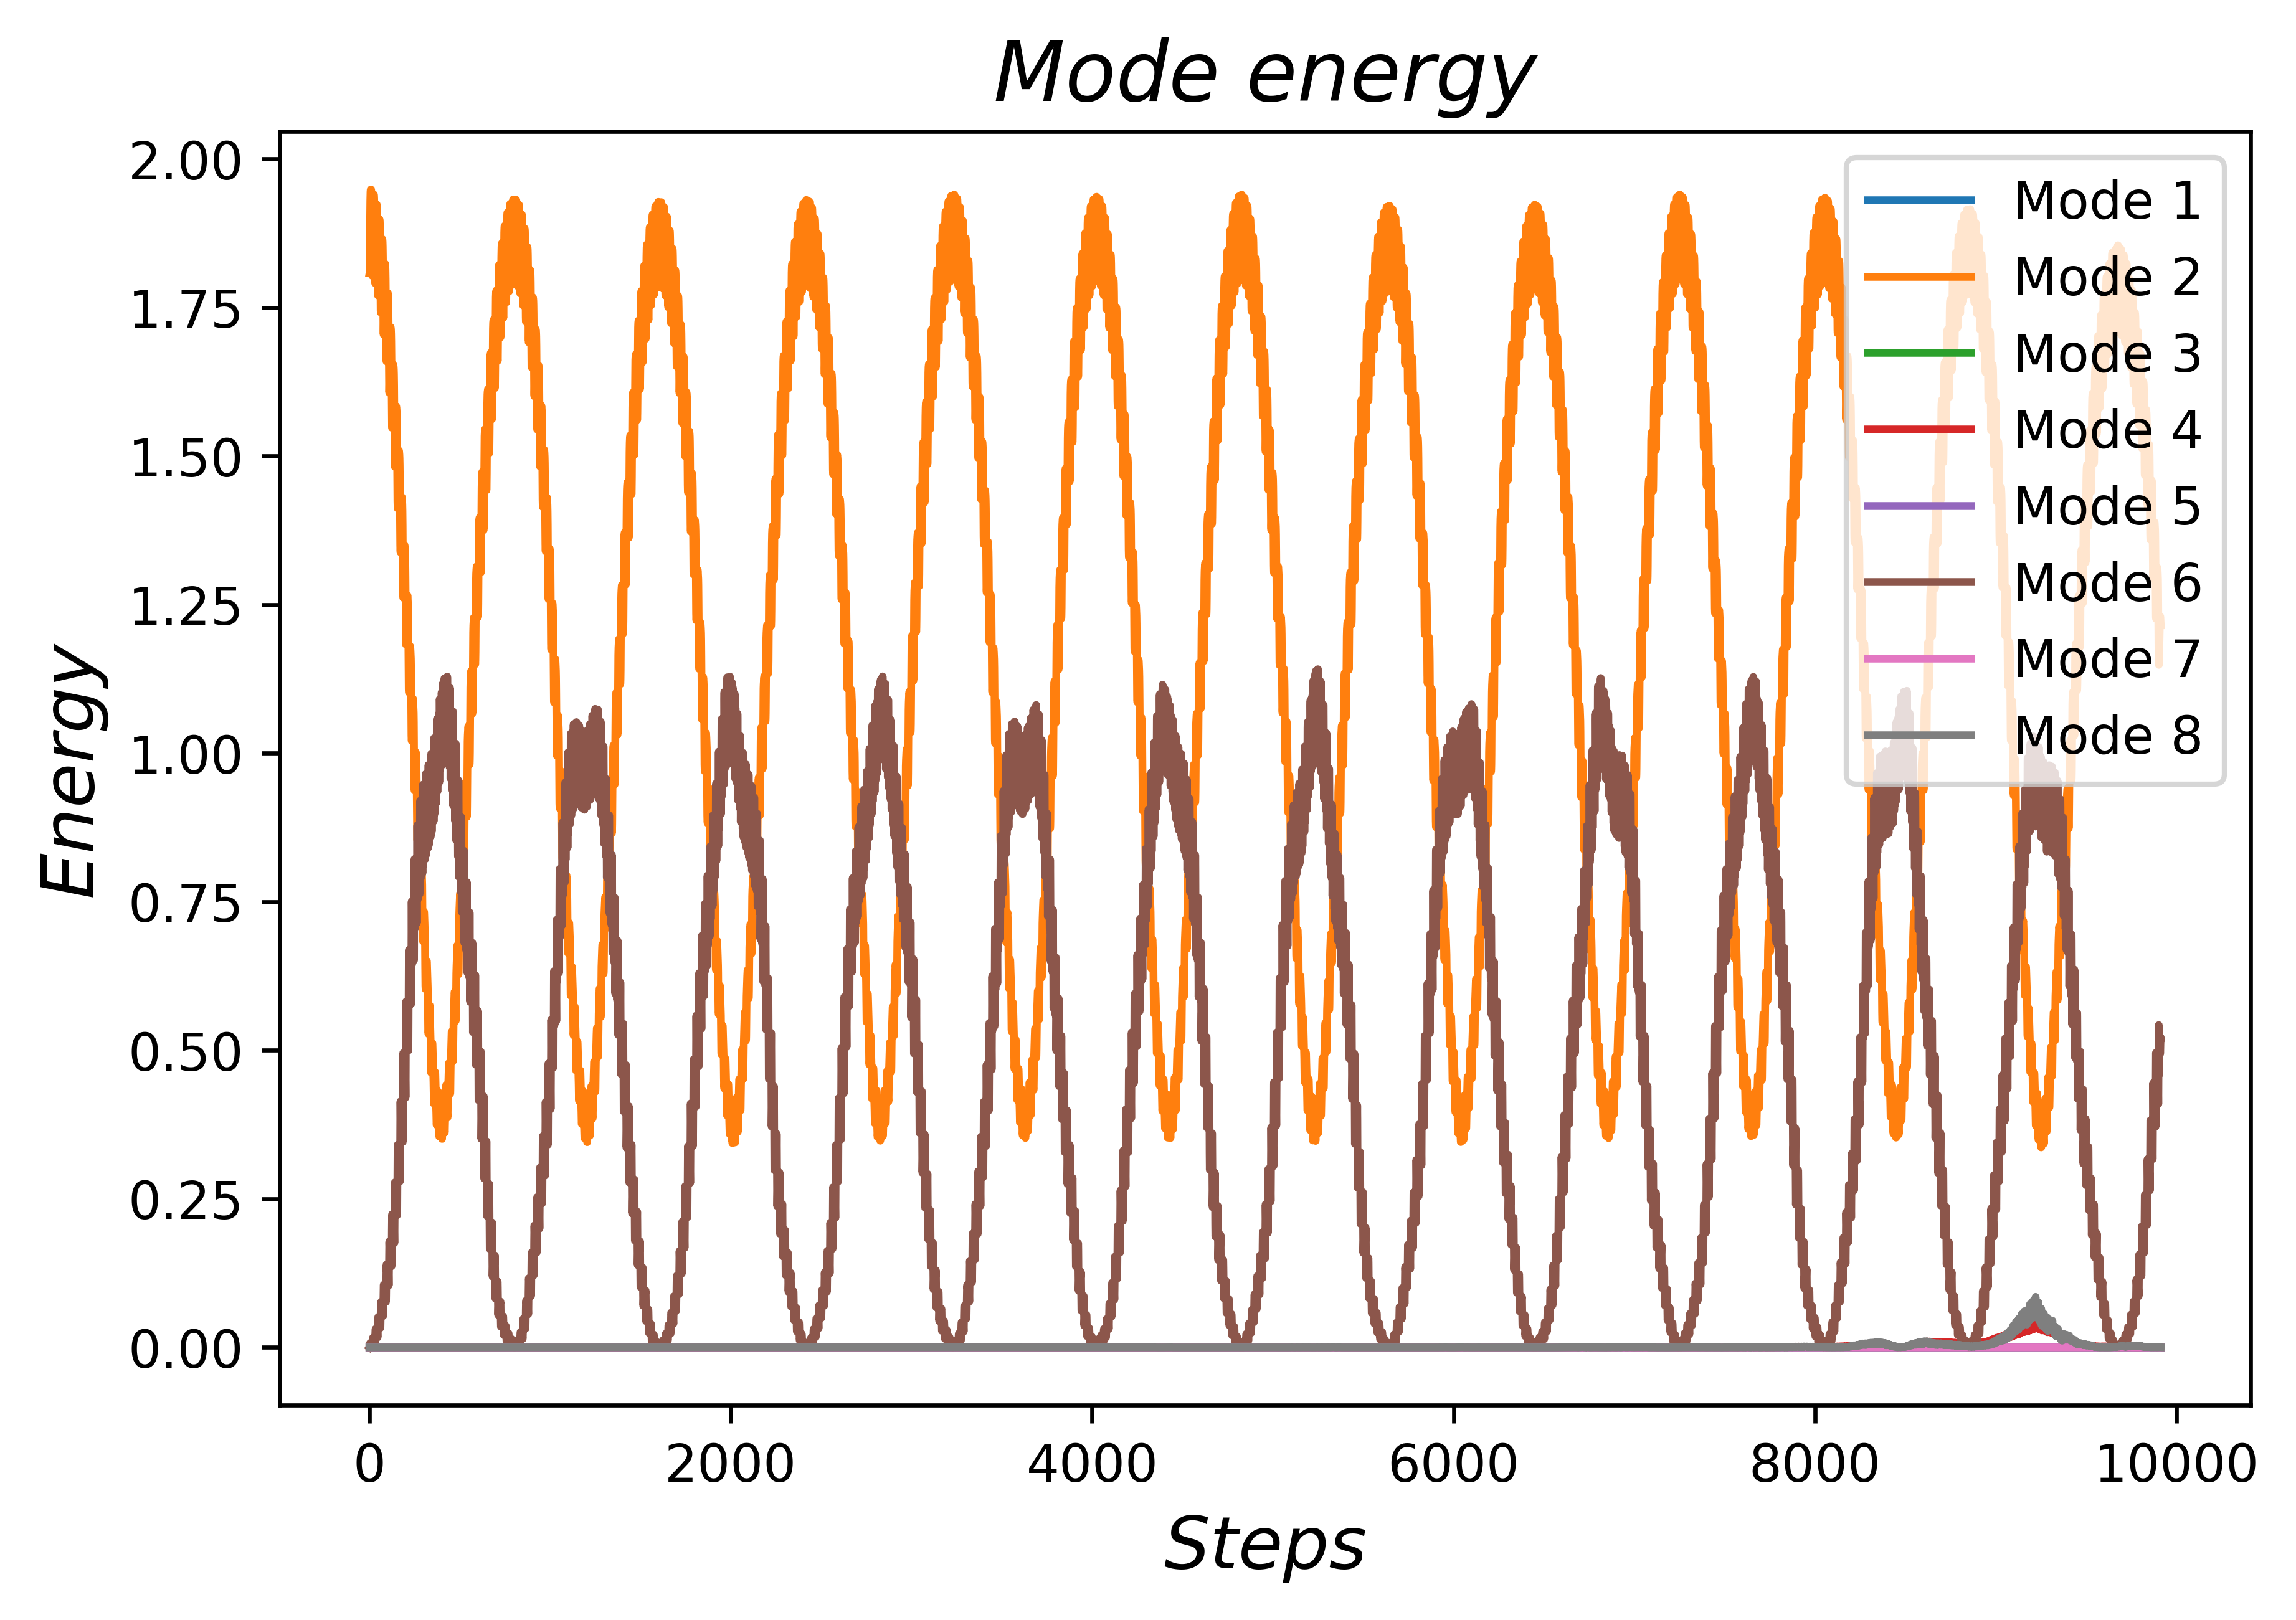
\includegraphics[scale=.53]{EnergiesN=2B=1}
\small{This plot shows the super-recurrence observed in the $\ell=2$ $\beta=1$ system where the period of recurrence can be approximated to be $T\approx40$. Note that this number was determined by multiplying the steps by the time between each step (.05 seconds).}
\end{figure} 

Experiment two successfully demonstrated the FPU paradox by confirming that once a sufficient nonlinear factor was introduced into the system that super-recurrence occurred. With a nonlinear factor of $\beta=1$ and initializing mode of $\ell=1$, the period of super-recurrence was approximately $t=290=5800\times0.05$ (see Figure (2)) where 5800 is the number of steps and 0.05 is the time between each step. An interesting feature of the super-recurrence was in regards to which modes the energy dissipated into. Notably, the energy only dissipated into other odd numbered modes (i.e. $\ell=3$, $\ell=5$, ...) and at decreasing amounts (i.e. mode $\ell=3$ had more energy than $\ell=5$, etc.). This feature was also present when the initial mode was even numbered, where the energy dissipated into other even numbered modes with decreasing amounts (see Figure (5)).
\begin{figure}[ht!]
\centering
\caption{$\epsilon_{crit}$ vs $\beta$}
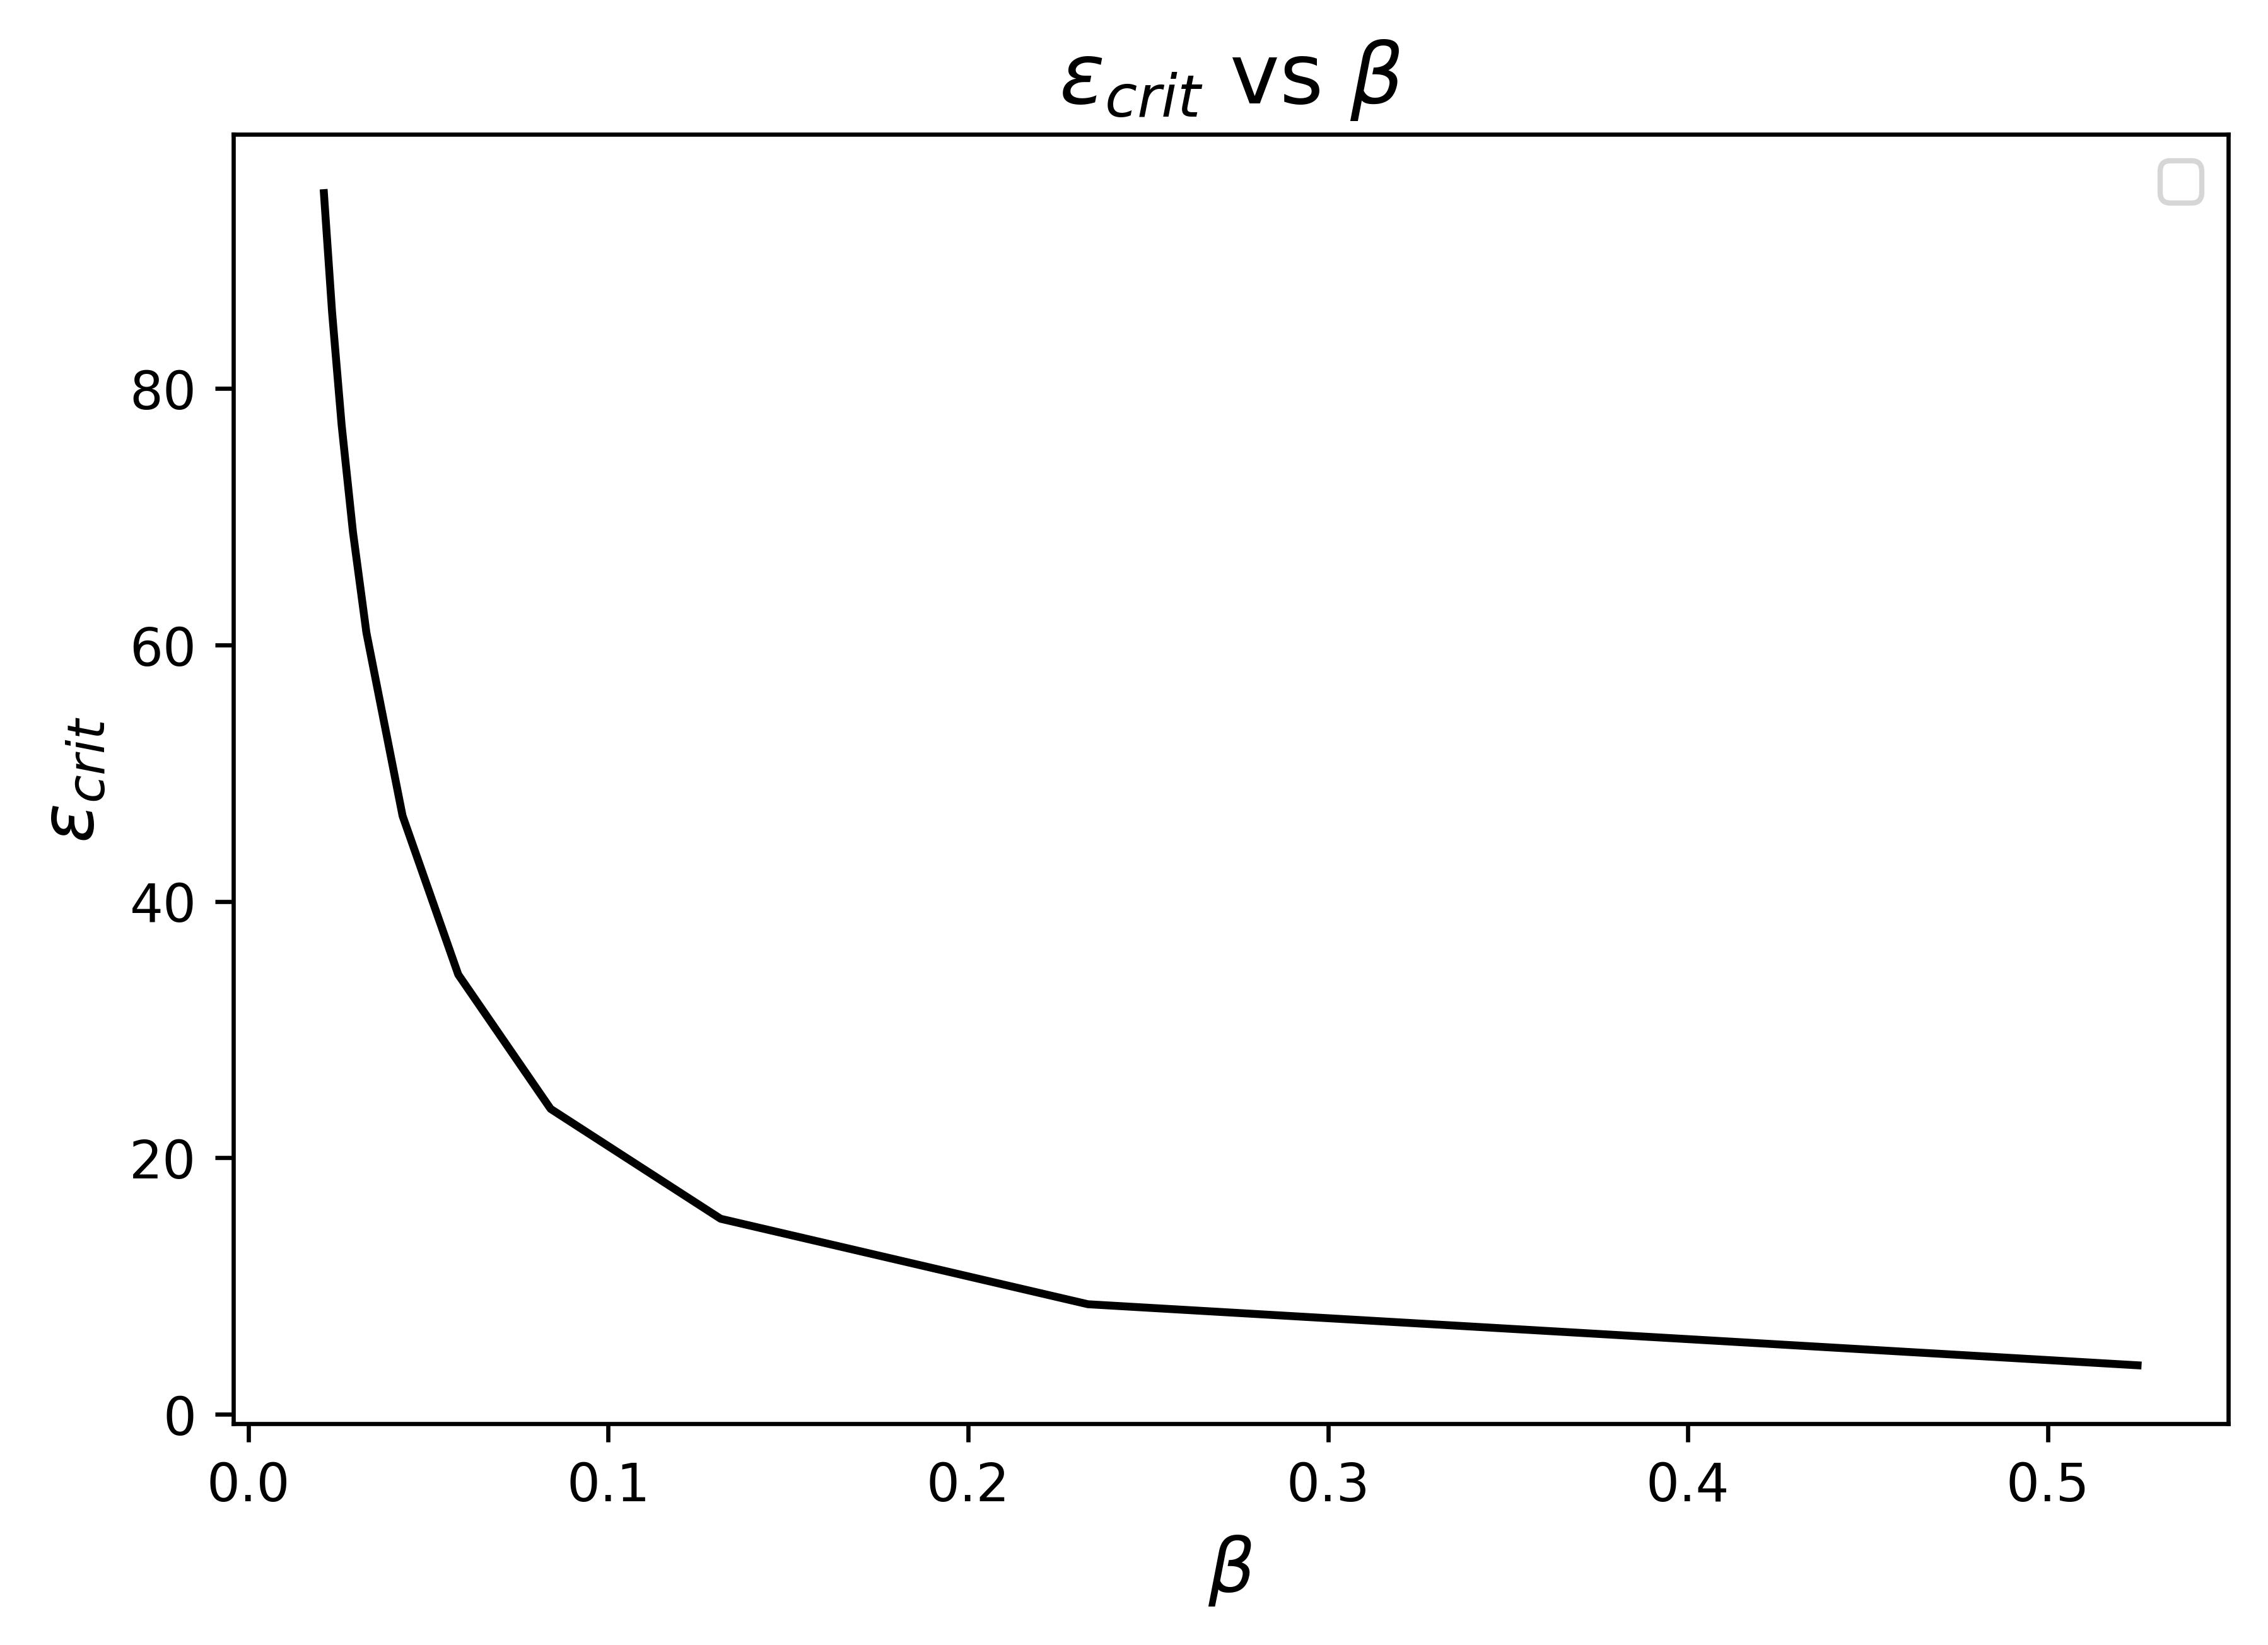
\includegraphics[scale=.55]{Q3a}
\small{This plot displays the exponential decay present in $\epsilon_{crit}$ as a function of $\beta$. This critical energy per mass is the point at which the system becomes ergodic.}
\end{figure}
\begin{figure}[ht!]
\centering
\caption{$\epsilon_{crit}$ vs $\beta$}
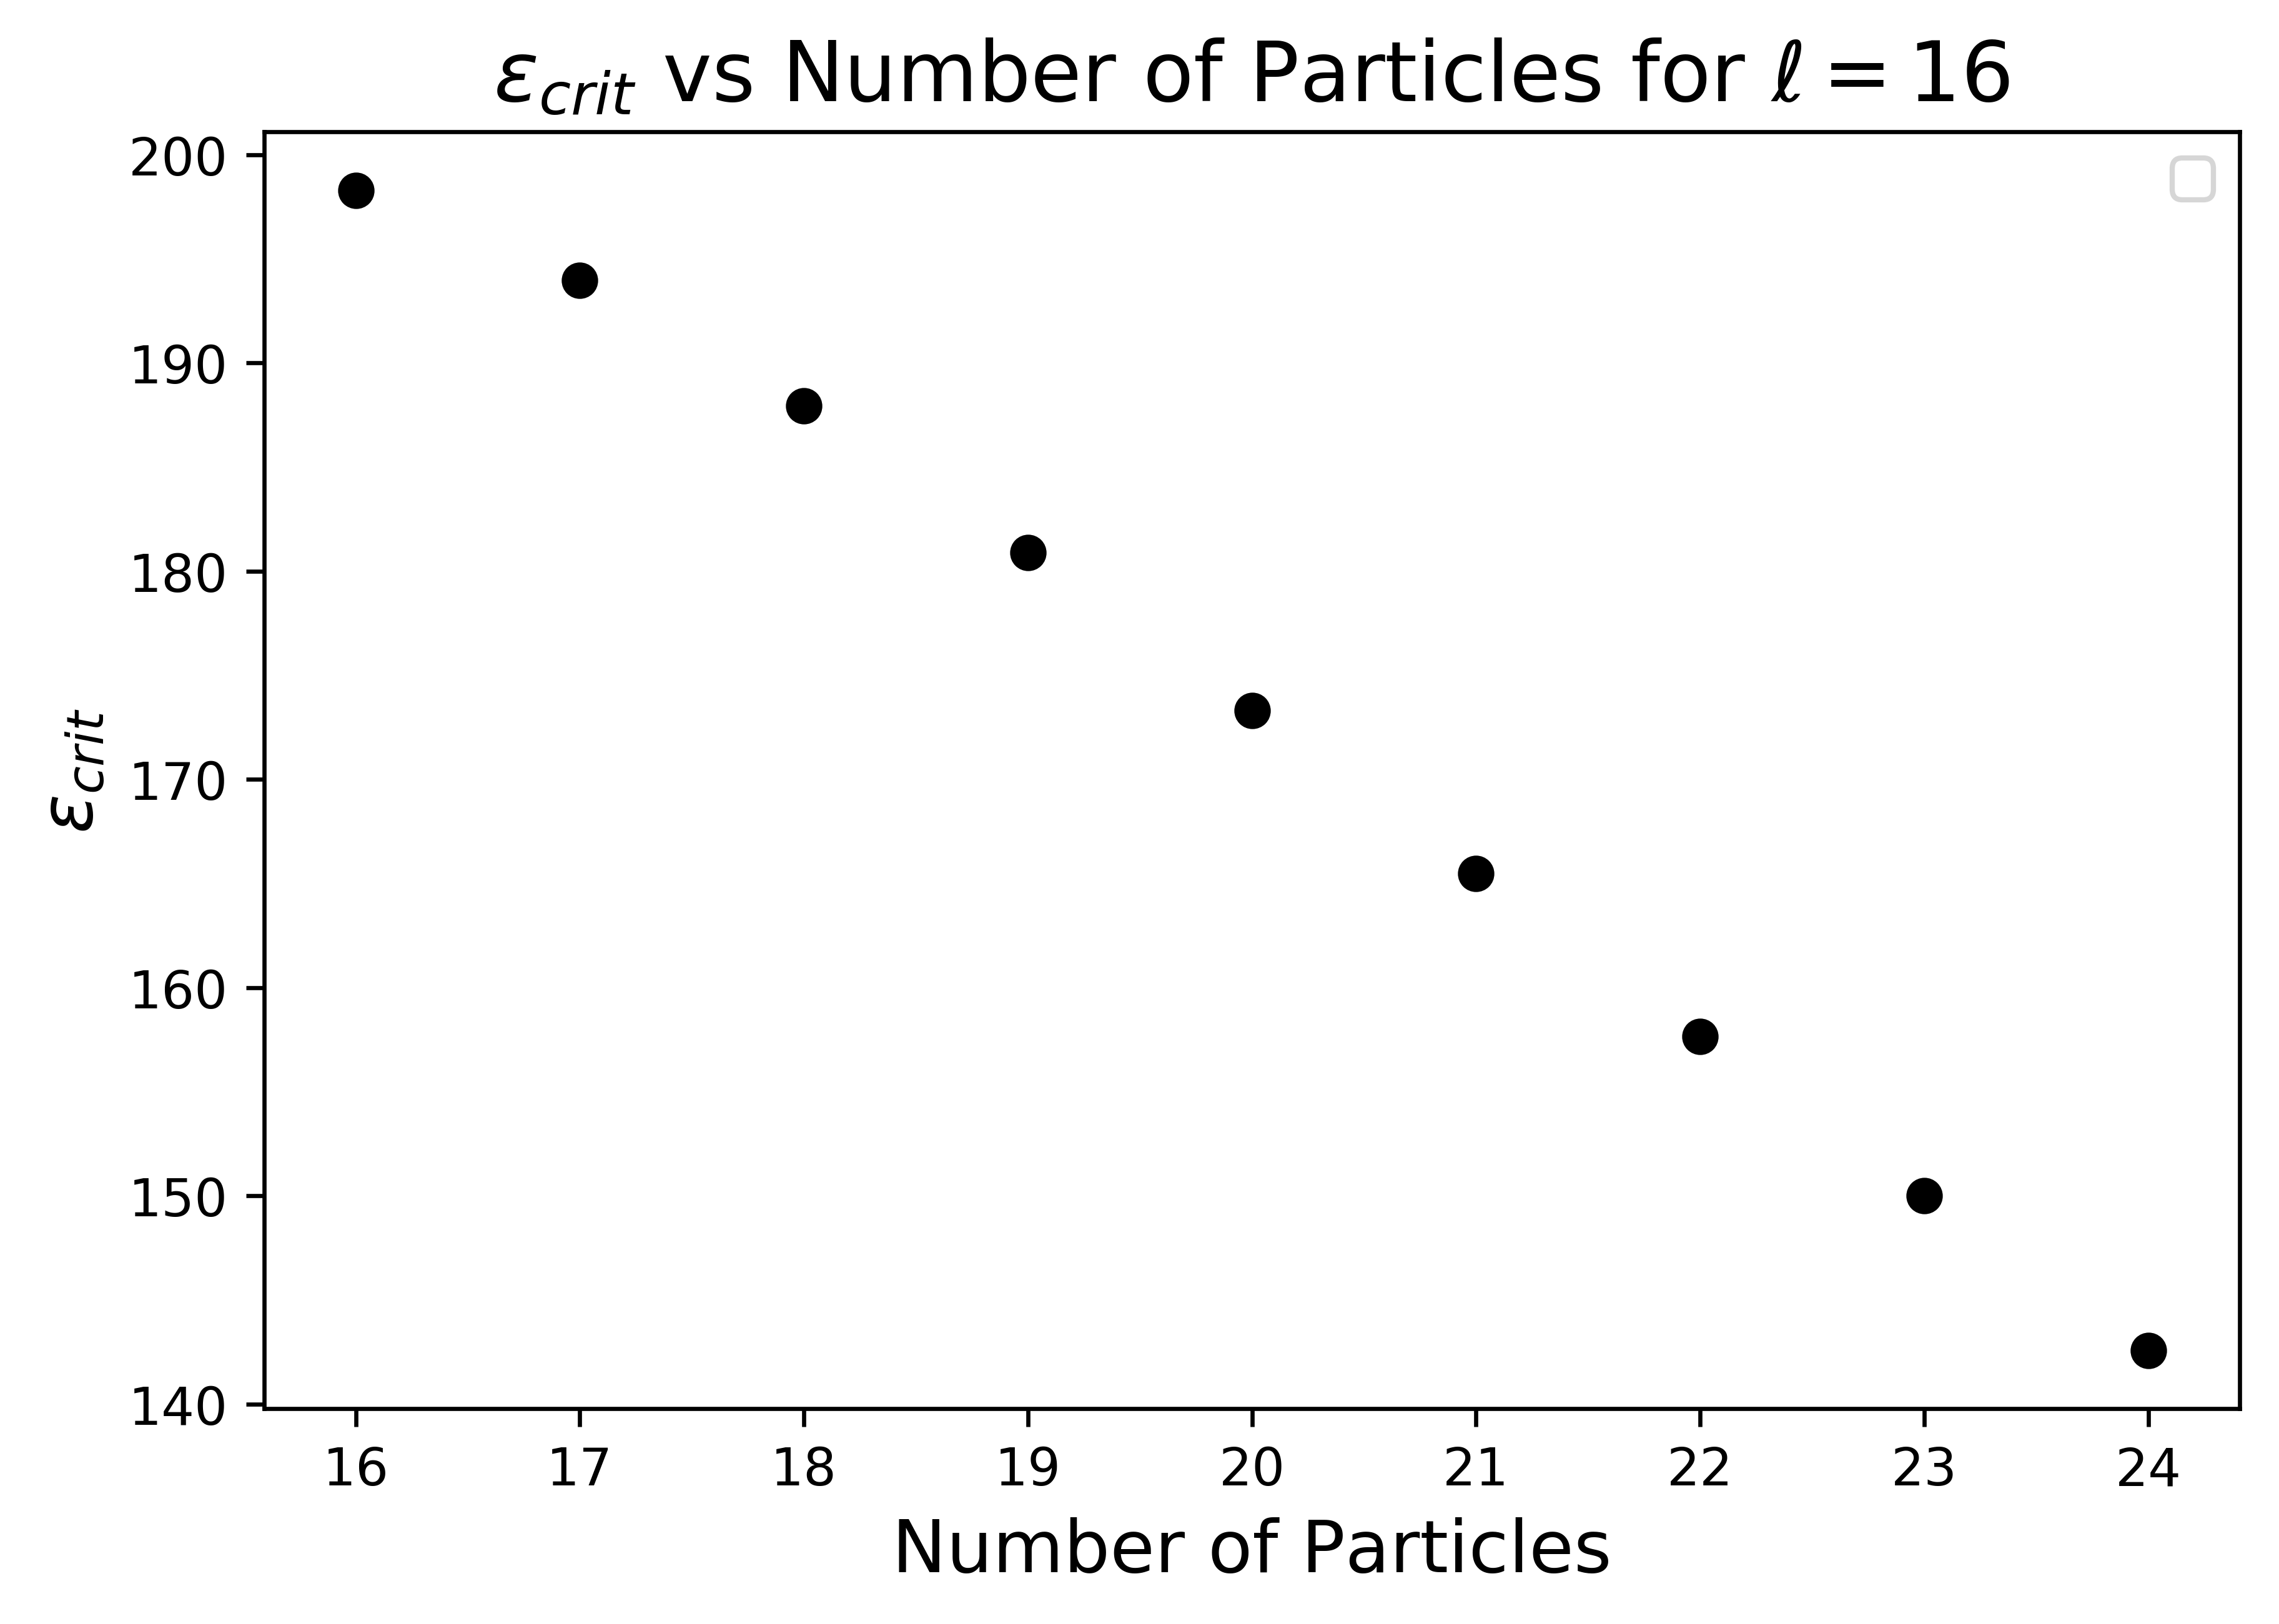
\includegraphics[scale=.55]{Q3b}
\small{This plot show the approximately linear decay present in $\epsilon_{crit}$ as a function of $N$. The linear decay was not necessarily predicted but after further considerations still sensible.}
\end{figure}

Experiment three proved very tricky to simulate but was ultimately successful. The standard deviation of the energy across all of the modes was shown to be periodic up to and prior $\beta=.02$, in the case that the system was initialized with $\ell=16$, after-which it was then shown to decay exponentially (see Figures (8) and (9)). Likewise, $\epsilon_{crit}$ was also shown to undergo exponentially decaying behavior as a function of $\beta$ (see Figure (6)). This behavior was expected; however, because the less energy per mass their is, the more nonlinearity there is required for any significant acceleration changes, and consequentially energy dissipations to occur. Similarly, the plot of $\epsilon_{crit}$ vs $N$ also experienced decay, but in an approximately linear manner (see Figure (7)). This behavior makes sense if one considers the definition of $\epsilon_{crit}$ defined in equation $(8)$, wherein $\epsilon_{crit}$ is affected by a factor of $\frac{1}{N}$ in addition to an initial energy that is also affected by $N$ in such a way that the result is a nearly linear decay.
\begin{figure}[ht!]
\centering
\caption{$\ell=16$ $\beta=0.01$}
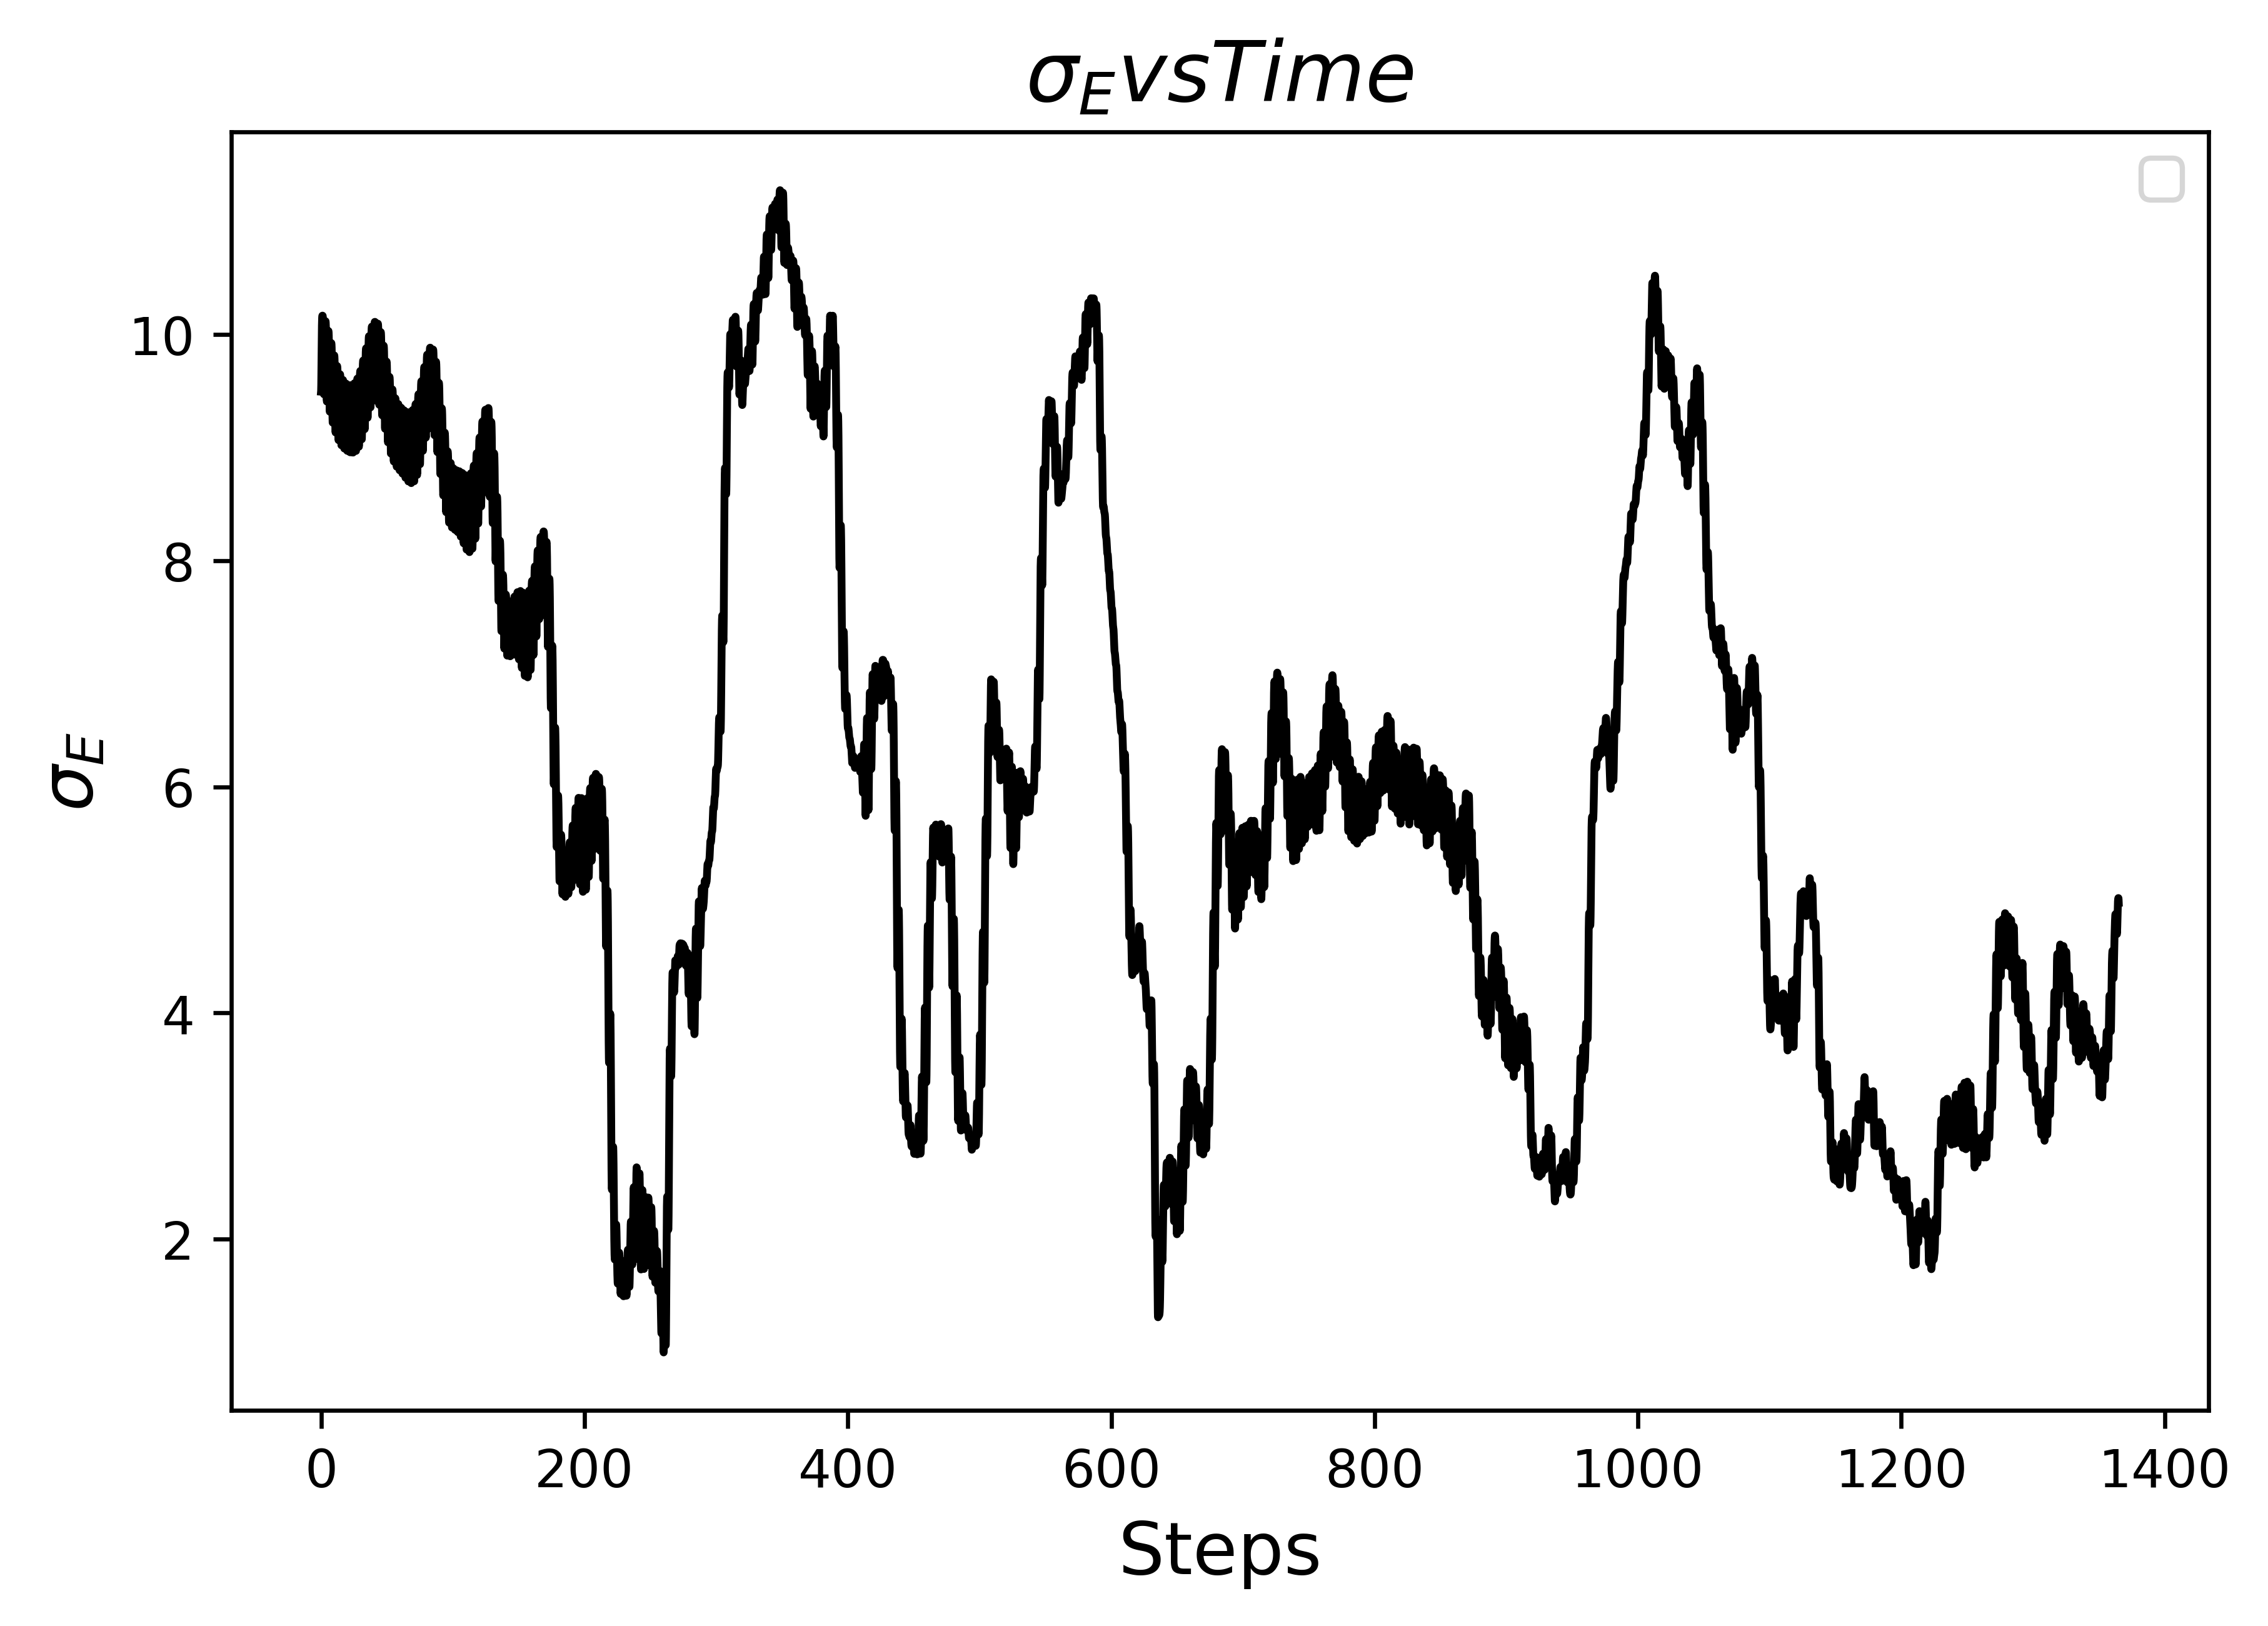
\includegraphics[scale=.55]{sigmaMode=16B=001}
\small{This plot shows the system $\ell=16$, where $\beta=0.01$ is less than the critical amount $\beta_{crit}$. Hence, the system is still behaving nonergodically and may exhibit super-recurrence.}
%\end{figure}
%\begin{figure}[ht!]
\centering
\caption{$\ell=16$ $\beta=0.02$}
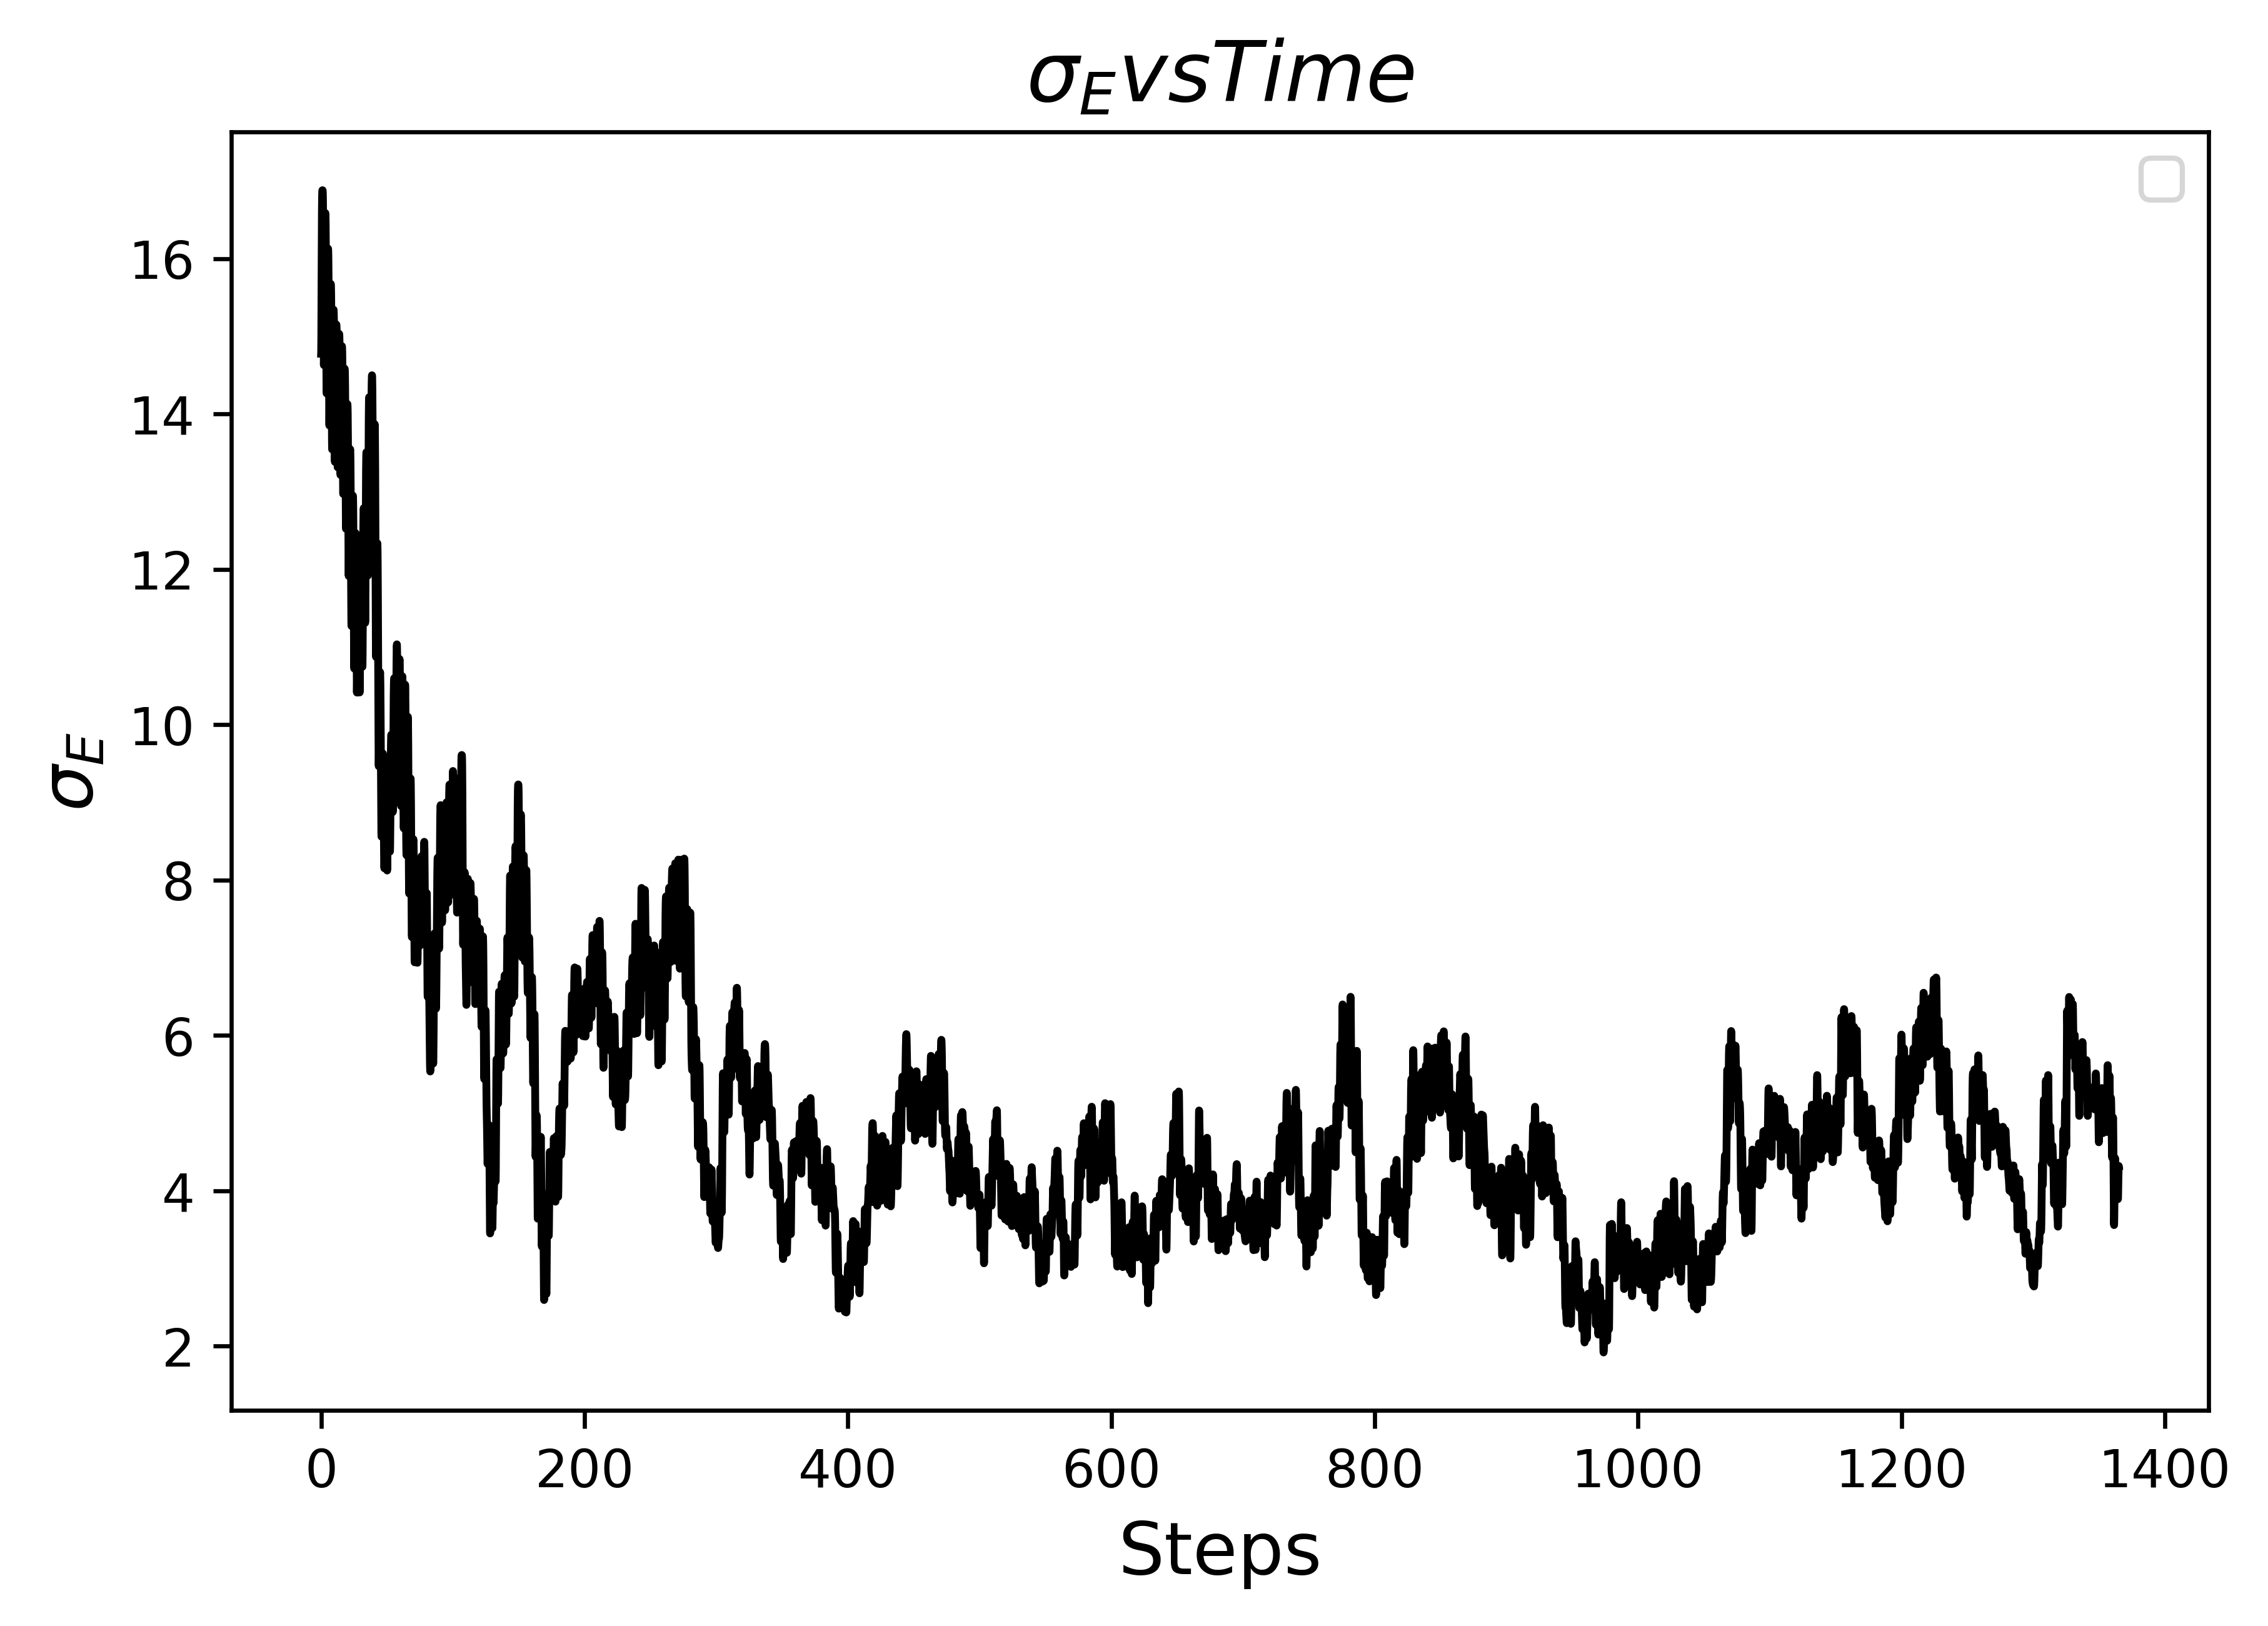
\includegraphics[scale=.55]{sigmaMode=16B=003}
\small{Unlike the plot above, this plot shows the same system except when $\beta=0.03$ is greater than the critical amount $\beta_{crit}$. Hence, $\sigma_E$ decreases exponentially because the system behaves ergodically.}
\end{figure}

Experiment four attempted to find other cases of super-recurrence outside of the $\ell=1$ mode by utilizing the formula for $\beta_{crit}$ and applying it to a new initialing mode. This process was performed for the initializing mode $\ell=2$ where the corresponding $\beta=1$ was less than $\beta_{crit}$. To no surprise, the plot exhibited super-recurrence as a function of the energy per mode vs time, since the system was initiated below $\beta_{crit}$ - the point at which the system would become ergodic. In this case the period of super-recurrence was found to be $T\approx 40=800\times0.05$ where the energy was transferred to $\ell=6$ before returning to $\ell=2$ (see Figure(5)). Overall then, the fourth experiment was successful.
\begin{figure}[ht!]
\centering
\caption{$\ell=1$ vs $\beta=1$}
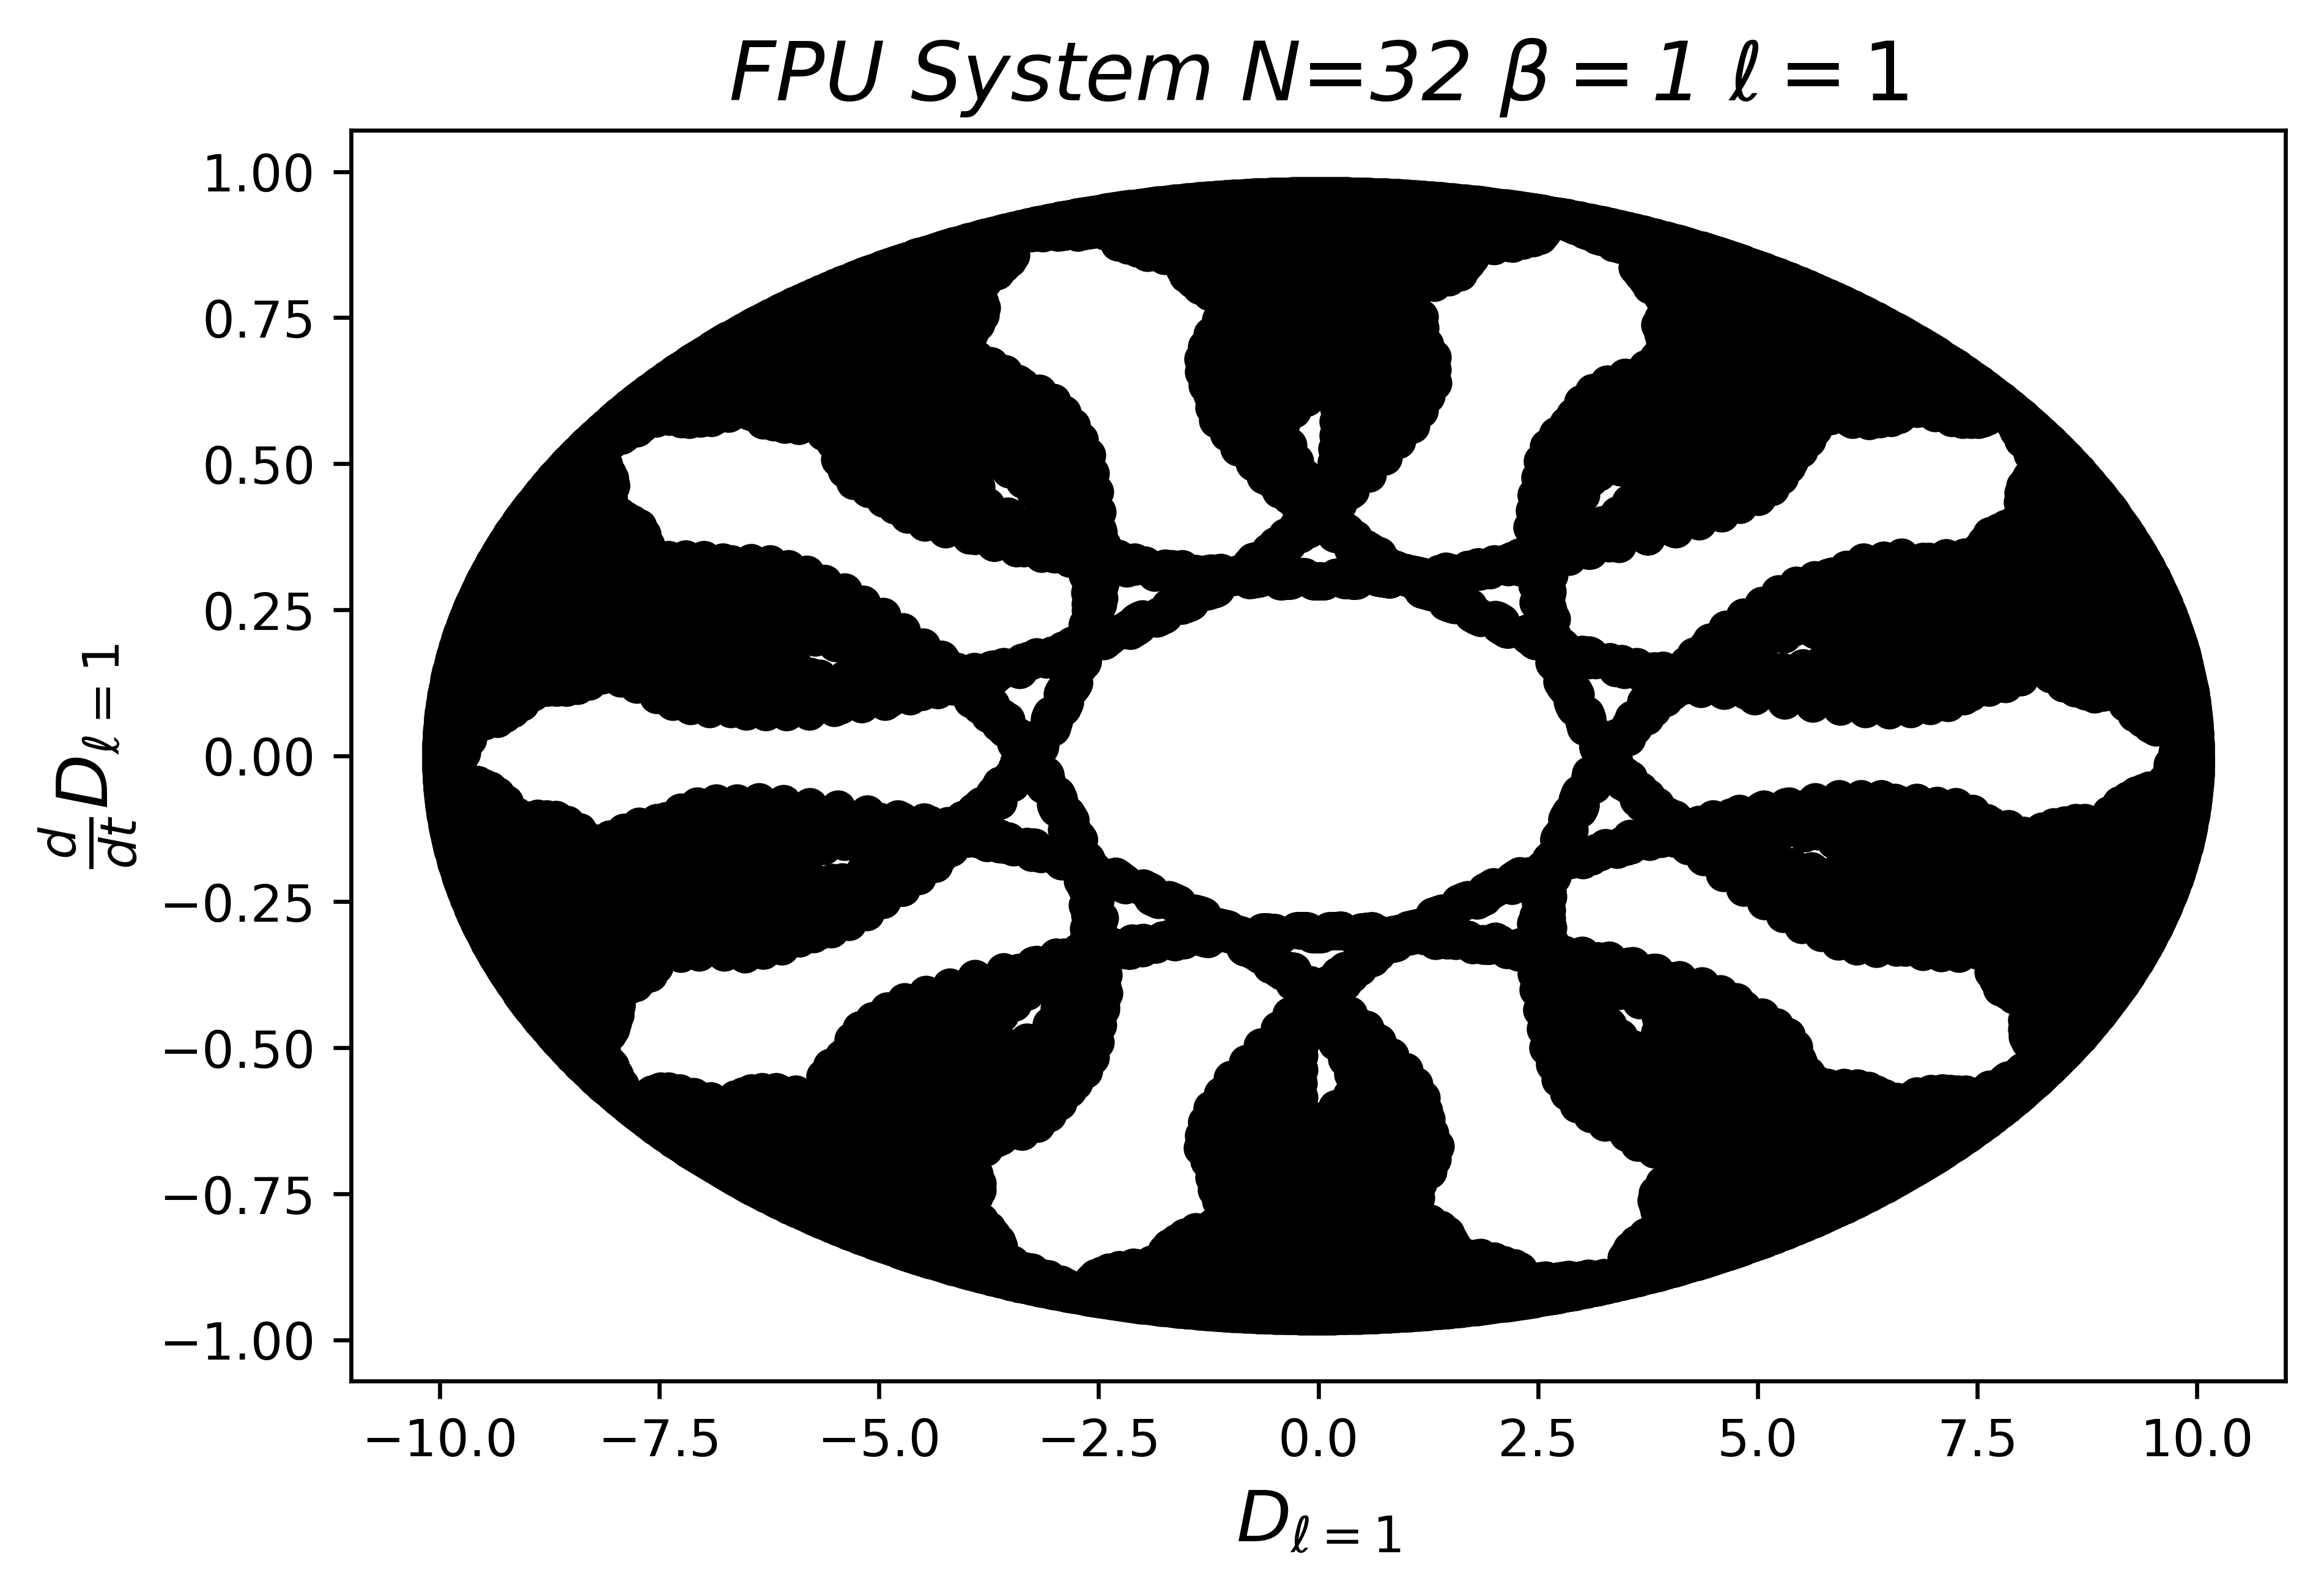
\includegraphics[scale=.5]{Poincare5bN=1B=1}
\small{This plot shows a Poincare section constructed by plotting $\frac{d}{dt}A_{\ell=1 }$ versus $A_{\ell=1}$} whenever $A_{\ell=5}=0$ for the system $\ell=1$, $\beta=1$. 
\end{figure}

The final experiment involved reproducing specific Poincare sections from Giordano's \textit{'Computational Physics'} on page 299. The sections themselves were created by measuring $\frac{d}{dt}A_{\ell=1 }$ and $A_{\ell=1}$ whenever $A_{\ell=3}=0$ in the three cases where the system was initialized with a starting mode of $\ell=1$ and corresponding nonlinearity factors $\beta=.3$, $\beta=1$, and $\beta=3$. A point of interest that should be noted is that, although the produced sections accurately portrayed the results found by Giordano, the first two were also surrounded by a solid ring that was much less distinct in Giordano's (see Figures (11), (12), and (13)). However, this is very likely a result of different intervals being used to trigger data recording - which was $-.1<A_{\ell=3}<.1$ in the program used for this paper.

Other unique Poincare sections were also created to examine the effects of a different trigger. The new trigger was set to record $\frac{d}{dt}A_{\ell=1 }$ and $A_{\ell=1}$ whenever $A_{\ell=5}=0$ in the cases where the initiating mode was $\ell=1$ with $\beta=1$ and where the initiating mode was $\ell=3$ with $\beta=.45$. The first case (see Figure (10)) produced a spectacular decagon surrounded by other unique structures and the second case (see Figure (4))created a fascinating spiral. Needless to say then, this trigger in conjunction with different starting modes and nonlinearity factors produced much different Poincare sections than the former ones.
\section{Conclusion}
In conclusion, each of the experiments produced results that were either identical or nearly identical to the results that other papers have published. In this sense the overall experiment was certainly a success. Some important highlights included: 
\begin{itemize}
\item demonstrating the FPU paradox when the system was initialized at $\ell=1$ with $\beta=1$ and approximating the period of super-recurrence
\item discerning the distinctions between $\sigma_E(t)$ both before and after $\beta_{crit}$ was reached - where prior to $\beta_{crit}$ the system was nonergodic and afterward it became ergodic
\item displaying how $\epsilon_{crit}$ decayed exponentially as a function of $\beta$ and how $\epsilon_{crit}$ decayed approximately linearly as a function of $N$
\item confirming that excited systems outside of the $\ell=1$ case can also show super-recurrence behavior if provided an appropriate $\beta$
\item reproducing Poincare sections from Giordano's \textit{'Computational Physics'}, which reaffirmed the accuracy of the program used to generate the results of all of the other plots in this paper
\item generating custom Poincare sections to observe other structures that can result from different recording triggers
\end{itemize}
\begin{figure}[h]
\caption{$\ell=1$ vs $\beta=.3$}
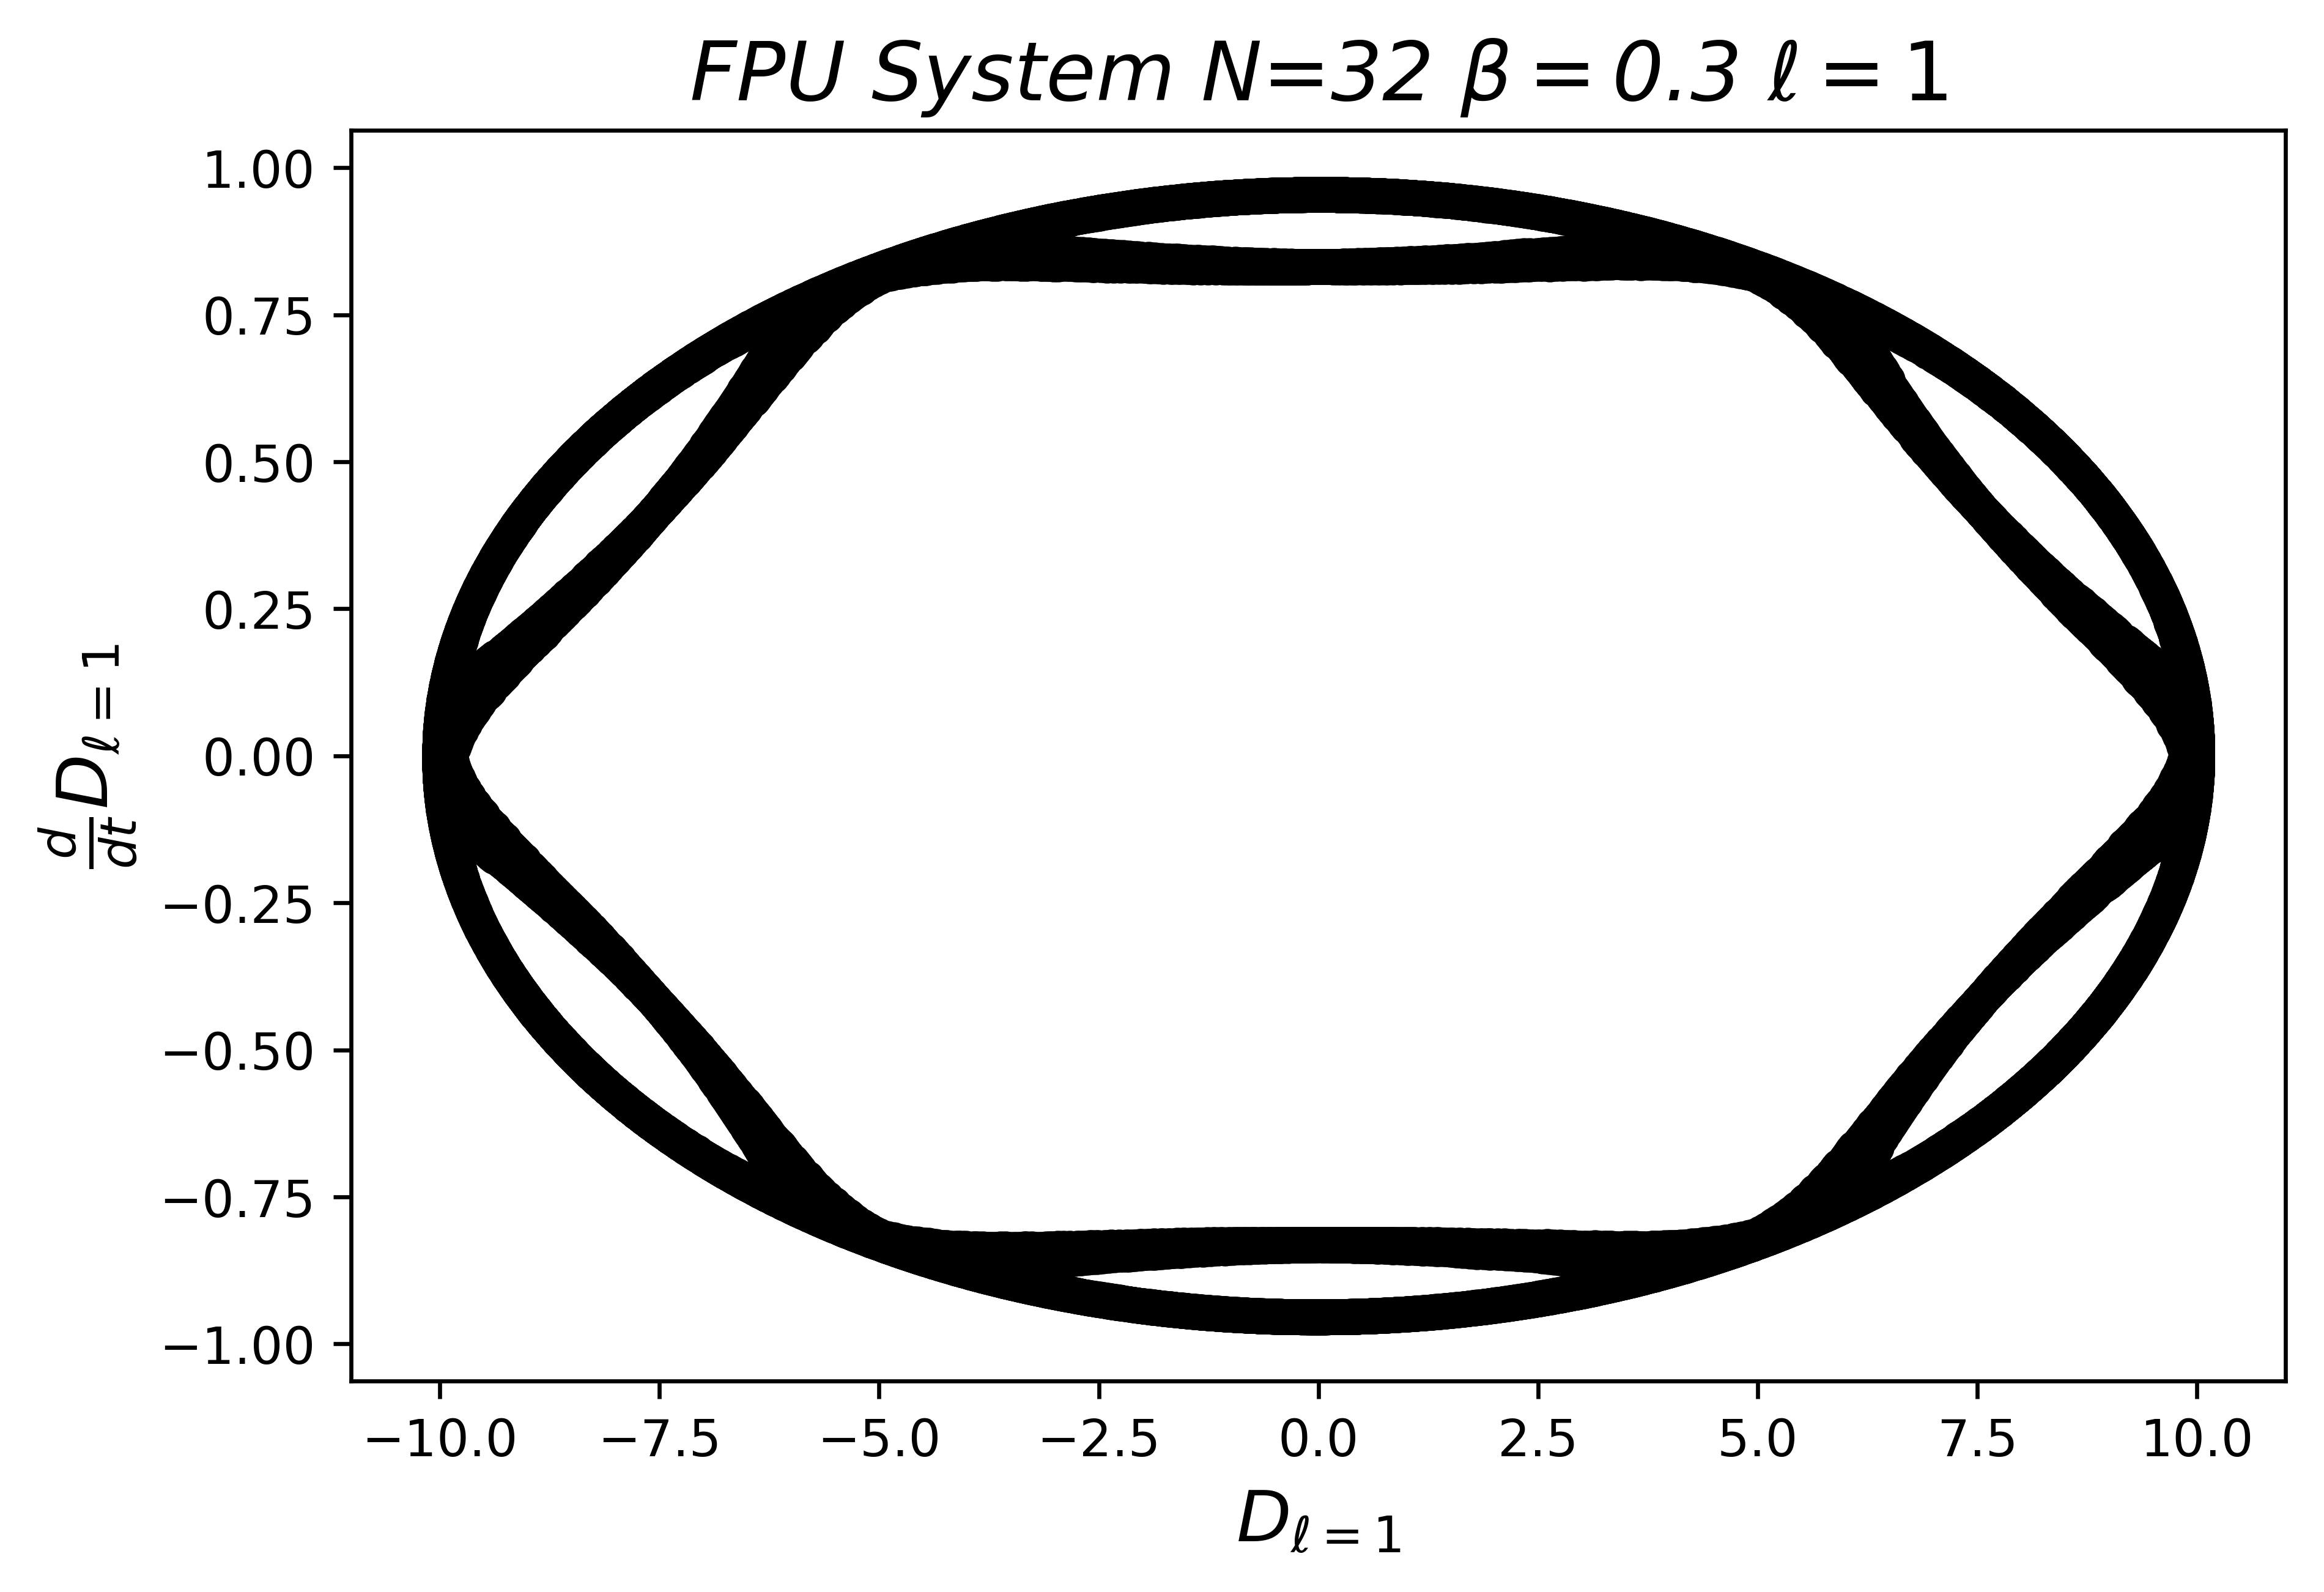
\includegraphics[scale=.55]{Poincare5aN=1B=003}
\caption{$\ell=1$ vs $\beta=1$}
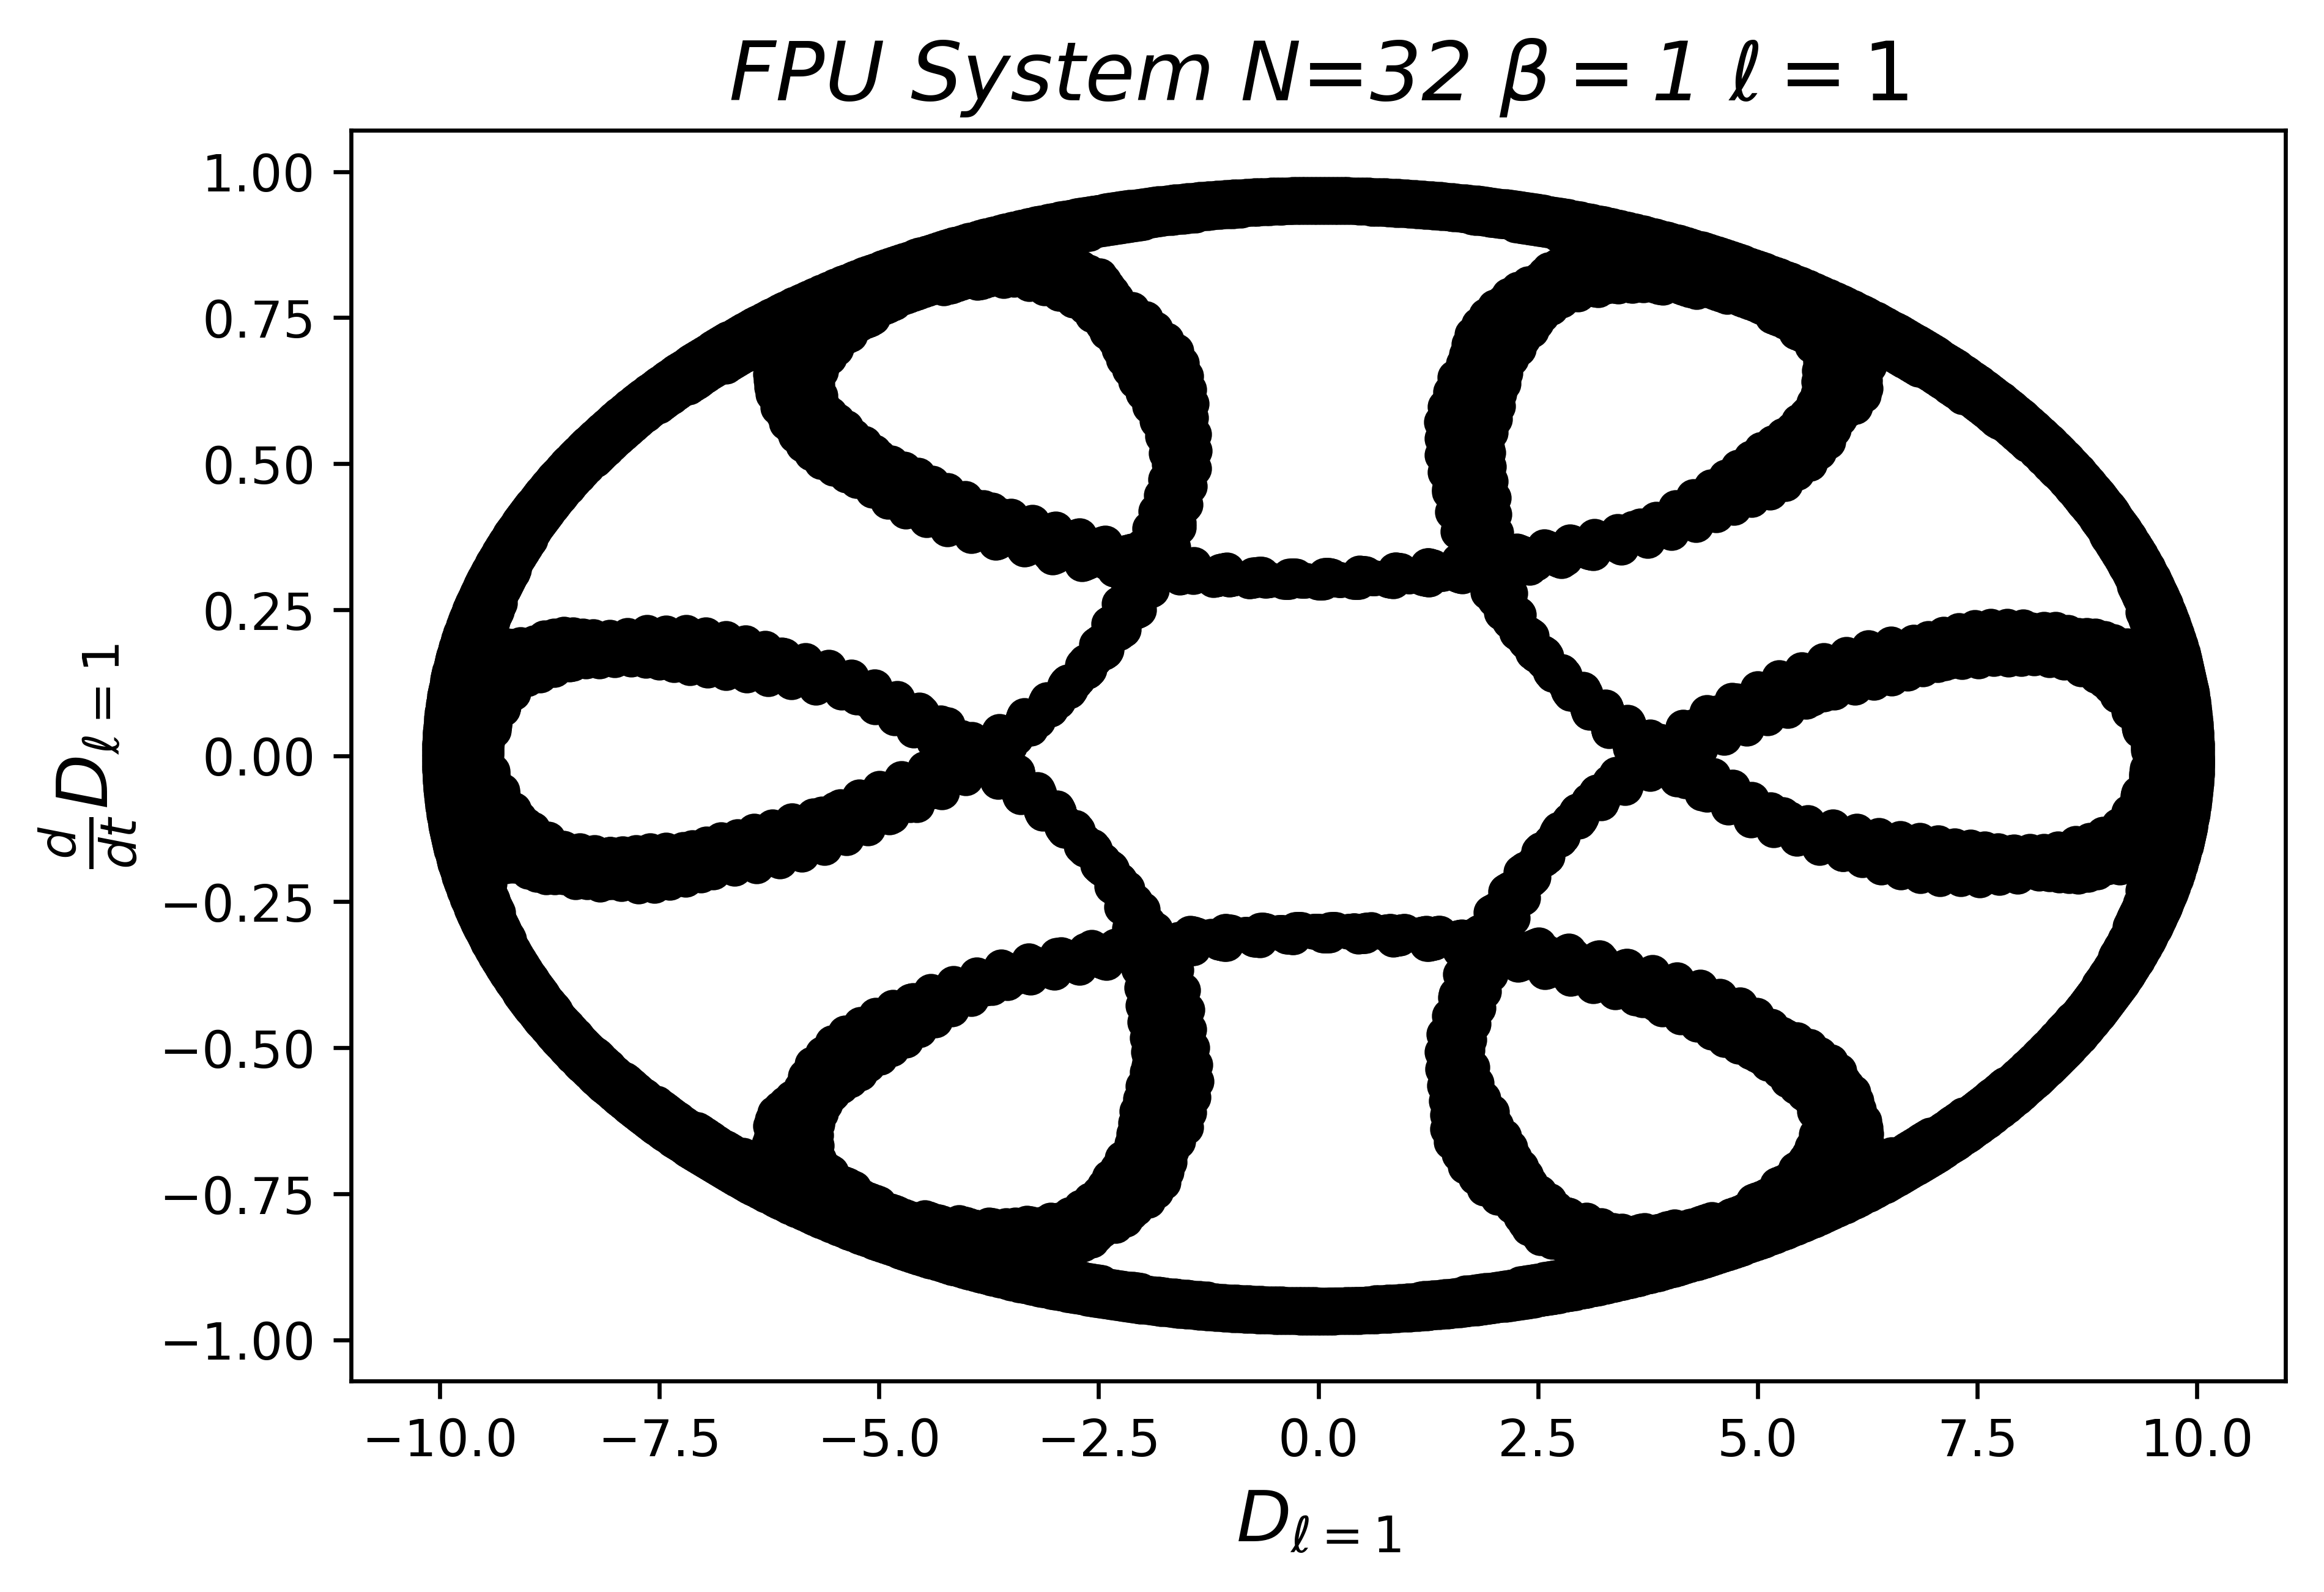
\includegraphics[scale=.55]{Poincare5aN=1B=1}
\caption{$\ell=1$ vs $\beta=3$}
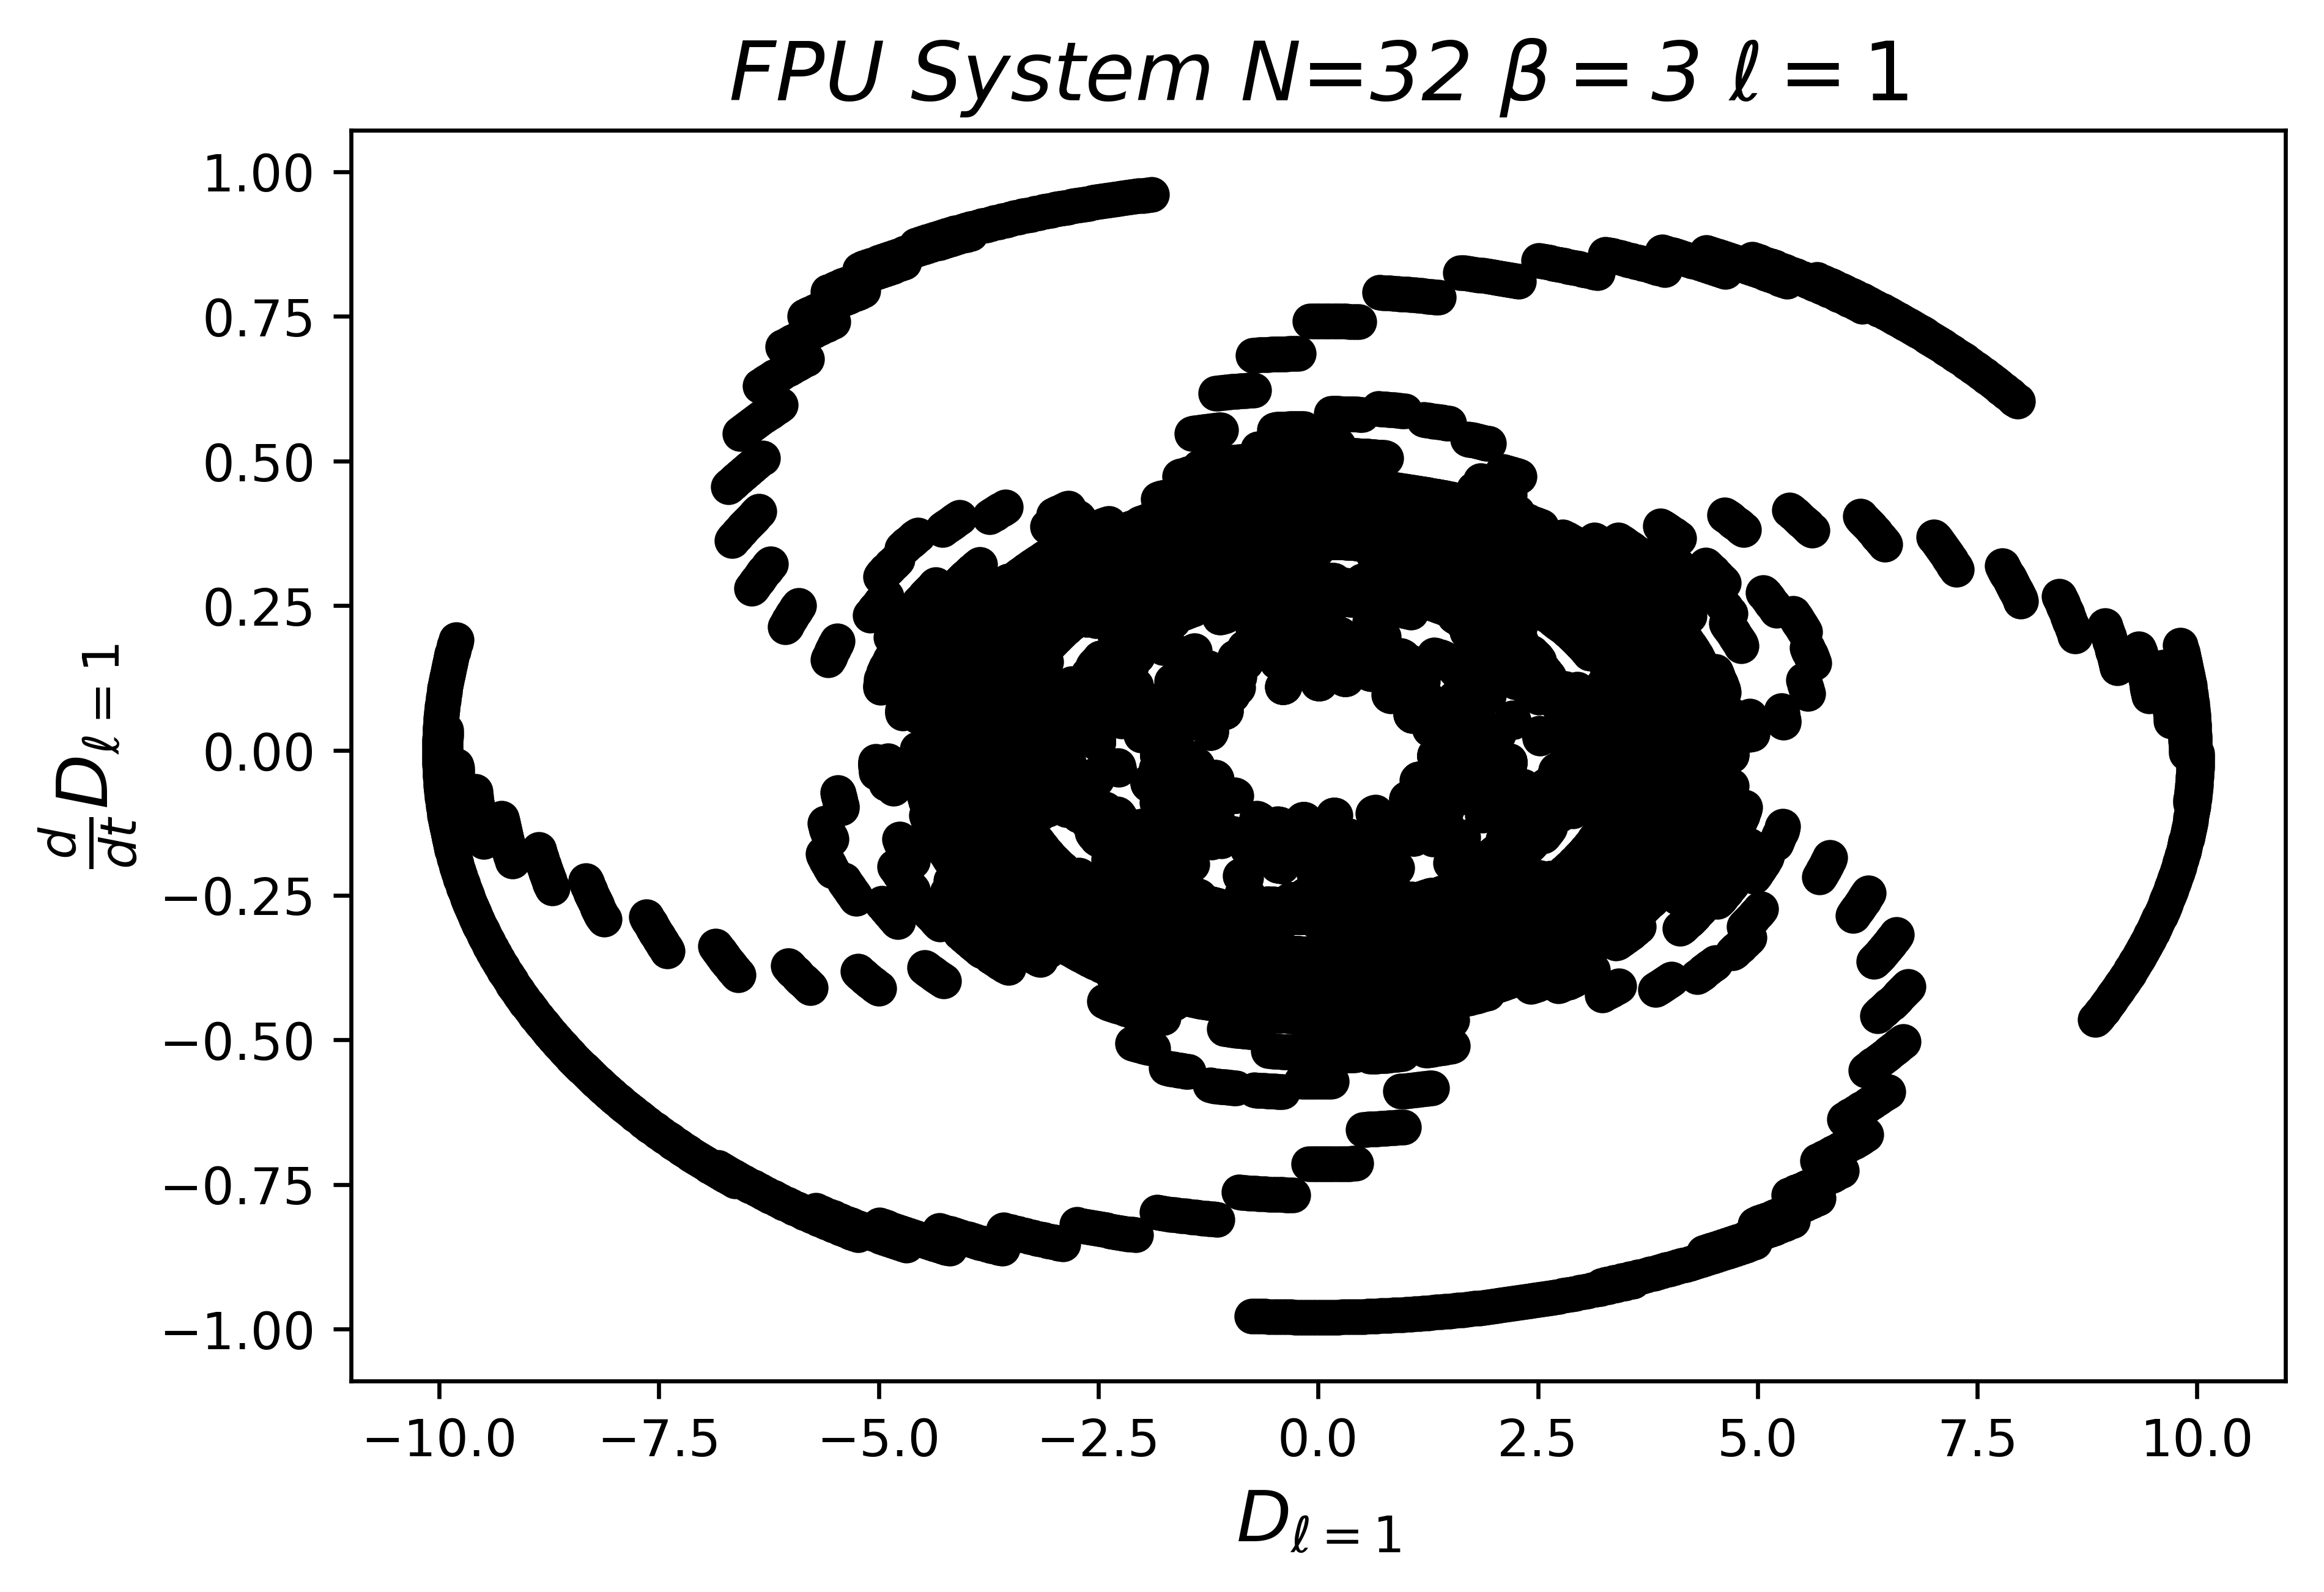
\includegraphics[scale=.55]{Poincare5aN=1B=3}
\centering
\small{These plots are recreations of the ones created in Giordano's \textit{'Computational Physics'} on page 299. They confirm that Giordano's work is verifiable}
\end{figure}

Most notable of all the conclusions of this paper though, has to be the confirmation of the FPU paradox - that ''nonlinearity is not sufficient to guarantee the equipartition of energy''$^{[2]}$ - which was arguably demonstrated the best in the third experiment where different nonlinearity factors introduced to the system were shown to only cause ergodic behavior above a certain $\beta_{crit}$. In other words, only specific nonlinearity factors resulted in the equipartition of energy. On a final note, it is worth considering that although many phenomena involving the classic FPU-$\beta$ model were explored in this paper, there still exists many other unsolved and open questions relating to it - such as 'How does the recurrence time scale with the system size?'$^{[1]}$ - that are open to the scientific community at large. 
%%%%%%%%%%%%%%%%%%%%%%%%%%%%%%%%%%%
% New Section
%%%%%%%%%%%%%%%%%%%%%%%%%%%%%%%%%%%
\begin{thebibliography}{9}
\bibitem{latexcompanion} 
\textit{''The Fermi-Pasta-Ulam problem: 50 years of progress''}
G. P. Berman and F. M. Izrailev
\bibitem{latexcompanion} 
\textit{''The Fermi Pasta Ulam ‘numerical experiment’: history and pedagogical perspectives''}. 
T. Dauxois, M. Peyrard, and S. Ruffo,
(2004).
\end{thebibliography}
\end{document}